% concatenated from main.tex
\documentclass[11pt]{amsart}

\usepackage[
backend=biber,
style=alphabetic,
sorting=nyt
]{biblatex} %Imports biblatex package
\addbibresource{bibtex.bib} 
%Import the bibliography file
\usepackage{enumerate}

\RequirePackage[utf8]{inputenc}
\usepackage{amsmath,amssymb}
\usepackage{amsfonts}
\usepackage{amsthm}
\usepackage{latexsym}
\usepackage{tikz}
\usetikzlibrary{shapes.geometric, arrows}
\usetikzlibrary{patterns}
\usepackage{graphicx}
\usepackage{epsfig}
\usepackage{enumerate}
\usepackage{xcolor}
\usepackage{hyperref}
\newtheorem{theorem}{Theorem}[section]
\newtheorem{lemma}[theorem]{Lemma}
\newtheorem{proposition}[theorem]{Proposition}
\newtheorem{definition}[theorem]{Definition}
\newtheorem{corollary}[theorem]{Corollary}
\newtheorem{claim}{Claim}[section]
\newtheorem{conjecture}{Conjecture}
\newtheorem{example}{Example}

\newtheorem{prop}{Proposition}[section]
\newtheorem{remark}[prop]{Remark}

%\newenvironment{proof}[1][Proof]
    %      {\medbreak\noindent {\em #1. \enspace}}
        %  {\enspace q.e.d. \par \medbreak}
%\newenvironment{definition}[1][Definition]
   %        {\medbreak\noindent {\em #1. \enspace}}
      %     {\par \medbreak}
%\newenvironment{remark}[1][Remark]
 %          {\medbreak\noindent {\em #1. \enspace}}
  %         {\par \medbreak}
\newenvironment{remarks}[1][Remarks]
           {\medbreak\noindent {\em #1. \enspace}} {\par \medbreak}
\makeatletter \@addtoreset{equation}{section} \makeatother
\renewcommand{\thesection}{\arabic{section}}
\renewcommand{\thesubsection}{\thesection.\arabic{subsection}}
\renewcommand{\theequation}{\thesection.\arabic{equation}}
\renewcommand*{\bibfont}{\footnotesize} % Change to desired size, e.g., \small, \scriptsize
\def\vol{\mathrm{vol}}
\def\av{\mathrm{Av}}
\def\dv{\mathrm{dV}}
\def\d{\mathrm{d}}
\def\div{\mathrm{div}}
\def\ric{\mathrm{Ric}}
\def\ddt{\frac{d}{dt}}
\def\ppt{\frac{\partial}{\partial t}}
\def\PP{{\mathbb P}}
\def\RR{{\mathrm R}}
\def \2R{{\hat{\RR}}}
\def\WW{{\mathrm W}}
\def\AA{{\mathrm A}}
\def\BB{{\mathrm B}}
\def\DD{{\mathrm D}}
\def\EE{{\mathrm E}}
%\def\EE{{\mathrm \dot{Rc}}}
\def\HH{{\mathrm H}}
\def\TT{{\mathrm{T}}}
\def\Rc{{\mathrm {Rc}}}
\def\oRc{{\overline{\mathrm {Rc}}}}
\def\Scal{{\RRR}}
\def\SS{{\mathrm S}}
\def\CC{{\mathrm C}}
\def\Rm{{\mathrm {Rm}}}
\def\He{{\mathrm{Hess}}}
\def\Re{\mathrm{Re}}
\def\QQ {\mathbb{Q}}
\def\diag{\mathrm{Diag}}
\def\id{\mathrm{Id}}
\def\det{\mathrm{det}}
\def\lie{\mathcal{L}}
\def\xi{\partial_{x_i}}
\def\yi{\partial_{y_i}}
\def\tr{\text{tr}}
%\pagestyle{plain}
\def\signature{\dotfill}

\usepackage[margin=1.5 in]{geometry}
%\setlength{\oddsidemargin}{0.25in}  % 1.25in left margin
%\setlength{\evensidemargin}{0.25in} % 1.25in left margin (even pages)
%\setlength{\topmargin}{0.0in}       % 1in top margin
%\setlength{\textwidth}{6.0in}       % 6.0in text - 1.25in rt margin
%\setlength{\textheight}{8.5in}      % Body ht for 1in margins



\begin{document}

\title{A lower bound for the first non-zero basic eigenvalue on a singular Riemannian foliation}
\author{Bach Tran}
\address{University of Oklahoma\newline
\indent Department of Mathematics\newline
\indent 601 Elm Ave\newline
\indent Norman, OK, 73019-3103, USA}
\email{bach.n.tran-1@ou.edu}
\date{\today}
\begin{abstract}
    In this paper, we provide  the lower bounds of the first non-zero basic eigenvalue on a closed singular Riemannian manifold $(M,\mathcal{F})$ with basic mean curvature that depends on the given non-negative lower bound of the Ricci curvature of $M$ and the diameter of the leaf space $M/\mathcal{F}$.
    
    These can be regarded as generalized versions of the Zhong-Yang estimate and a generalized Shi-Yang's estimate for singular Riemannian foliations with basic mean curvature. We also provide a rigidity result corresponding to the generalized Zhong-Yang estimate, which is a generalized Hang-Wang rigidity for singular Riemannian foliations with basic mean curvature. More precisely, when the first basic eigenvalue $\lambda_1^B$ is equal to $\frac{\pi^2}{\d_{M/\mathcal{F}}^2} $, where $\d_{M/\mathcal{F}}$ is the diameter of the leaf space, $M$ is 
    isometric to a mapping torus of an isometry $\varphi:N\to N$ where $N$ is an $(n-1)$-dimensional Riemannian manifold of nonnegative Ricci curvature and $\mathcal{F}$ has the form $\{[\{\text{point}\}\times N]\}$.
\end{abstract}
\maketitle
\tableofcontents
\markboth{Bach Tran}{A lower bound for the first non-zero basic eigenvalue on a singular Riemannian foliation}

\section{Introduction}\label{00000}

The study of how curvature influences the eigenvalues of the Laplacian has been a central theme in Riemannian geometry since the 1950s. One interesting problem in that trend is giving estimates for lower and upper bounds of the first eigenvalue of the Laplacian of a compact Riemannian manifold under curvature assumptions (in this paper, specifically, lower bounds on the Ricci curvature).

Recall that the Laplacian, or the Laplace-Beltrami operator on a Riemannian manifold $(M^n,g)$ is given by
$$\Delta=\div(\nabla).$$
A value $\lambda$ will be called an eigenvalue of the Laplacian of $M$ if there exists a non-zero function $f\in C^\infty(M)$ (that we call an  eigenfunction with the eigenvalue $\lambda$) such that 
$$\Delta f=-\lambda f.$$
When $M$ is compact, we know the fact that $\lambda$ is non-negative.

Let $\lambda_1(M)$ be the first non-zero eigenvalue of the Laplacian on $M$ and $\lambda_1$ if we are clear about which manifold we work on.




In the case that $\ric(M)\geq (n-1)K\geq 0$ for some constant $K$, many results have been found: Lichnerowicz \cite{lich} and Obata \cite{obata} proved that on a closed Riemannian manifold with $K>0$, one has $\lambda_1\geq nK$ and the equality holds if and only if $M$ is isometric to the $n$-sphere of radius $1/\sqrt{K}$. In the case $\ric(M)\geq 0$, we cannot get a positive lower bound without a restriction of the diameter $\d_M$ of $M$: for example, in the case of torus, if we increase the diameter arbitrarily and approaching infinity, then the first eigenvalue approaches $0$. Moreover, the diameter restriction is automatic in the case of $K>0$ by Bonnet-Myer's theorem. Hence, the diameter restriction is necessary. By Li and Yau \cite{liyau} and the improvement by Li \cite{li}, we get a gradient estimate for the first nontrivial eigenfunction and derive that
$$\lambda_1\geq\frac{\pi^2}{2\d_M^2}.$$

Zhong and Yang \cite{zhongyang} enhanced this result to be an optimal one for the case of $\ric(M)\geq 0$:
$$\lambda_1\geq \frac{\pi^2}{\d_M^2}.$$
Hang and Wang \cite{hangwang} later provided and proved the rigidity statemtent for Zhong-Yang estimate: the equality holds if and only if $M$ is isometric to a circle of radius $\d_M/\pi$. 

We can see there are many works about general optimal lower bound estimate for $\lambda_1$ for a given lower bound $(n-1)K$ of the Ricci curvature, for example, in \cite{progen,mufawang,benjulie,zhangwang}, and see also \cite{bakryqian,benni, yuehe,xashguoqi}. Inspired by foundational results of Lichnerowicz and Zhong-Yang, Li had conjectured that the first positive eigenvalue should satisfy the following estimate (see \cite{dagang})
\begin{align*}
    \lambda_1\geq\frac{\pi^2}{\d_{M}^2}+(n-1)K.
\end{align*}
The conjecture greatly motivates many related studies in this area and an effort to prove the so-called Li's conjecture will unify Zhong-Yang's estimate and Lichnerowicz's estimate. Many people tried to prove this conjecture, and in particular, some towards improved inequalities of the form
\begin{align}\label{aha}
    \lambda_1\geq\frac{\pi^2}{\d_{M}^2}+\alpha(n-1)K.
\end{align} for some constant $\alpha$ were made. A remarkable result by Shi and Zhang in \cite{shizhang} proved that for any $s\in (0,1)$
\begin{align*}
    \lambda_1\geq4s(1-s)\frac{\pi^2}{\d_M^2}+s(n-1)K.
\end{align*}
Notice that for $s=\frac{1}{2}$, we have a particular estimate
\begin{align*}
    \lambda_1\geq\frac{\pi^2}{\d_M^2}+\frac{1}{2}(n-1)K.
\end{align*} In \cite{benjulie}, B. Andrews and J. Clutterbuck showed that the inequality of this form \ref{aha} with $\alpha=\frac{1}{2}$ is the best possible constant and this means Li's conjecture is false. For more detail of the history, see \cite{yuehe}.





So how is the lower bound estimates of the first eigenvalue related to the object we will discuss in this paper, the first \textit{basic} eigenvalue on a singular Riemannian foliation? We first introduce the concept of singular Riemannian foliations. A singular Riemannian foliation on a Riemannian manifold $M$, roughly speaking, is a partition of $M$ into connected injectively immersed submanifolds (we call \textit{leaves}), which are locally equidistant to one another (see subsection \ref{121212}). One class of examples of singular Riemannian foliations are orbits of isometric actions of Riemannian manifolds, that we call \textit{homogeneous}. Another class of examples are connected components of the fibers of Riemannian submersions, that we call \textit{simple}. For more detail about homogeneous and simple singular Riemannian foliations, see \cite{radeschi}. 

Given $(M,\mathcal{F})$ a singular Riemannian foliation, we define $\mathcal{F}$-\textit{basic function}, is a function that is constant on each leaf of $\mathcal{F}$. When the know which $\mathcal{F}$ we talk about, we can call it briefly \textit{basic function}. This allows us to define $\mathcal{F}$-\textit{basic Laplacian} as an operator that sends basic smooth functions to basic smooth functions and define $\mathcal{F}$-\textit{basic eigenvalues}, that we will discuss more detail in Section \ref{121}. When $(M,\mathcal{F})$ admits a \textit{basic mean curvature}, it turns out that the ordinary Laplacian coincides with the basic Laplacian, and any results that work for the ordinary Laplacian can be used to derive corresponding results for the basic Laplacian. In the case of estimate a lower bound for the first non-zero basic eigenvalue $\lambda_1^B$, if we use Lichnerowiz's estimate, we can get $\lambda_1^B\geq \lambda_1\geq nK$ but it does not imply any better result because $nK$ does not depend on $\mathcal{F}$ that we consider, and we do not see the difference between Lichnerowicz's estimate for the first non-zero eigenvalue and Lichnerowic'z estimate for the first non-zero basic eigenvalue. However, for the estimates involving the diameter like in \cite{zhongyang,progen,mufawang,benjulie,zhangwang,shizhang}, we can generalize them by replacing the diameter $\d_M$ of the ambient manifold $M$ with the diameter of the leaf space $\d_{M/\mathcal{F}}$ and it is reasonable to expect similar estimates with leaf space diameters. Hence, in this paper, we assume that the Ricci curvature of the ambient manifold is bounded below by a non-negative value. 

In the case of non-negative Ricci curvature, we obtain a generalized version of Zhong-Yang estimate for singular Riemannian foliations
        \begin{theorem}\label{main1}

    Let $M^n$ be a compact Riemannian manifold with non-negative Ricci curvature and $\mathcal{F}$ a singular Riemannian foliation of $M$ with closed leaves and basic mean curvature. Then we have a lower bound for the first non-zero basic eigenvalue $\lambda_1^B$ of the Laplacian, given by \begin{align}
        \lambda_1^B\geq \frac{\pi^2}{d_{M/\mathcal{F}}^2}.
    \end{align}
\end{theorem}

We also have the rigidity of Theorem \ref{main1}, that generalize Hang-Wang result as the following
\begin{theorem}\label{main2}
    Let $M^n$ be a connected compact Riemannian manifold with non-negative Ricci curvature and $\mathcal{F}$ a singular Riemannian foliation of $M$ with closed leaves and basic mean curvature. Assume that $\lambda_1^B=\frac{\pi^2}{\d_{M/\mathcal{F}^2}}$. Then $M$ is isometric to $\mathbb{R}\times_\mathbb{Z}N$, where $N$ is a compact $(n-1)$-dim Riemannian manifold with $\ric\geq 0$ and $\mathbb{R}\times_\mathbb{Z}N=(\mathbb{R}\times N)/\mathbb{Z}$ with the isometric action of $\mathbb{Z}$ is defined by $k\cdot (t,x)=\left(t+\frac{2k\pi}{\sqrt{\lambda_1^B}},\varphi^k(x)\right)$ where $k\in \mathbb{Z},(t,x)\in \mathbb{R}\times N$ and $\varphi:N\to N$ is an isometry of $N$. Furthermore, $\mathcal{F}$ is a (regular) Riemannian foliation of codimension $1$ of the form $\{[\{\text{point}\}\times N]\}$.

    Consequently, $M/\mathcal{F}$ is isometric to the circle of radius $\frac{1}{\sqrt{\lambda_1^B}}$.
\end{theorem}

Notice that in this theorem,  $\mathbb{R}\times_\mathbb{Z}N=\left[0,\frac{2\pi}{\sqrt{\lambda_1^B}}\right]\times N/\sim$, where  $(0,x)\sim\left(\frac{2\pi}{\sqrt{\lambda_1^B}},\varphi(x)\right),\forall x\in N$, is exactly a space so-called a \textit{mapping torus} of $\varphi:N\to N$.



Finally, we have the generalized version of Shi-Zhang estimate for singular Riemannian foliations when we have a non-negative lower bound of the Ricci curvature
\begin{theorem}
   \label{main}
    Let $M^n$ be a compact Riemannian manifold and $\mathcal{F}$ a singular Riemannian foliation of $M$ with closed leaves and basic mean curvature. Assume the Ricci curvature of $M$ is bounded below by $(n-1)K\geq 0$. Suppose $\lambda_1^B$ is the first non-zero basic eigenvalue of $(M,\mathcal{F})$. Then
    \begin{align}\label{uuuuuu}
        \lambda_1^B\geq 4s(1-s)\frac{\pi^2}{d_{M/\mathcal{F}}^2}+s(n-1)K,
    \end{align}for any constant $s$ such that $0<s<1$.
    

    
\end{theorem}
\begin{remark}Notice that when $\mathcal{F}$ is a foliation by points, $M/\mathcal{F}$ is just the same as the ambient manifold $M$, and we recover Zhong-Yang estimate, Hang-Wang rigidity, and Shi-Zhang estimate. In the more general case, when $\mathcal{F}$ is given as the (connected) fibers of a Riemannian submersion $\pi:M\to M/\mathcal{F}$ with totally geodesic (or, more generally, minimal) fibers, the basic spectrum of $M$ is turned out to be the spectrum of the base $M/\mathcal{F}$ of the submersion and $\lambda_1^B$ is the first non-zero eigenvalue $\alpha_1$ of the base $M/\mathcal{F}$, we get Theorem \ref{main1} by applying the Zhong-Yang estimate directly for $\alpha_1=\lambda_1^B$  of the base $M/\mathcal{F}$. However, we cannot apply Hang-Wang rigidity or Shi-Zhang estimate for the base to get Theorem \ref{main2} or Theorem \ref{main} respectively. These points will be discussed more detail in sections \ref{ililil} and \ref{1111}.
\end{remark}
\begin{remark}
    Particularly, in the case of small diameter of $M$, we can choose a specific value of $s$ to get the optimal estimate:
    \begin{align*}
        \lambda_1^B\geq\frac{\pi^2}{\d_{M/\mathcal{F}}^2}+\frac{1}{2}(n-1)K+\frac{(n-1)^2K^2\d_{M/\mathcal{F}}^2}{16\pi^2}.
    \end{align*}

    We will discuss more after proving Theorem \ref{main} in Section \ref{1111}.
\end{remark}





The paper is structured as follows: in Section \ref{121}, we recall the main definitions and important results that we will use throughout the paper. In Section \ref{122}, we discuss some examples to illustrate Theorem \ref{main}. In Section \ref{7777}, we prove Theorem \ref{main1} and Theorem \ref{main2}. Finally, in Section \ref{1111}, we prove Theorem \ref{main}.


\textbf{Acknowledgements.} I would like to thank Dr. Ricardo Mendes, my Ph.D advisor, for many great ideas and suggestions of readings. His thoughtful feedback on my drafts, especially the discussion after the proof of Theorem \ref{main}, was greatly helpful in improving this paper. Also, I would like to thank Dr. Ken Richardson and Dr. Catherine Searle for comments on the last version of the rigidity statement in my last talk, it helped me figuring out how to state and prove the rigidity statement of Theorem \ref{main2} correctly. And thank Dr. Michael Jablonski and Dr. Marco Radeschi for comments and suggestion of writing on the latest version.





\section{Preliminaries}\label{121}
\subsection{Singular Riemannian Foliations}\label{121212}
\subsubsection{Basic definitions and facts}
Singular Riemannian foliations, first introduced in \cite{molino} by Molino in his study of Riemannian foliations and constitute nowadays an active field of research. 
\begin{definition}\label{667}
    Let $\mathcal{F}$ be a decomposition of a Riemannian manifold $(M,g)$ into connected injectively immersed submanifolds, called \textit{leaves}, which may have different dimensions. We say that $\mathcal{F}$ is a \textit{singular Riemannian foliation} if the following conditions are satisfied:
    \begin{enumerate}[(i)]
        \item $\mathcal{F}$ is a \textit{transnormal system}, that is, every geodesic orthogonal to one leaf remains orthogonal to all the leaves that it intersects,
        \item $\mathcal{F}$ is a \textit{singular foliation}, that is, $T_pL=\{X_p:X\in\mathcal{X}_{\mathcal{F}}\}$ for every leaf $L$ in $\mathcal{F}$ and every $p\in L$, where $\mathcal{X}_\mathcal{F}$ is the module of smooth vector fields on the ambient manifold $M$ that are everywhere tangent to the leaves of $\mathcal{F}$.
    \end{enumerate}

   
\end{definition}

The first condition in Definition \ref{667} is equivalent to the leaves being locally equidistant, see \cite{radeschi}, Proposition 2.3. If every leaf of $\mathcal{F}$ is closed, we say $\mathcal{F}$ is \textit{closed}. In this case, the condition of local equidistance of leaves becomes the global equidistance of leaves.

For a given singular Riemannian foliation $(M,\mathcal{F})$, leaves form a space that we call the \textit{leaf space}, denoted by $M/\mathcal{F}$. More precisely, we define an equivalence relation on $M$ by saying that $x\sim y$ if $x$ and $y$ are in the same leaf $L_x\in\mathcal{F}$ containing $x$, and then the corresponding element of $M/\mathcal{F}$ is $[L_x]$. In addition, if the leaves are closed, then because of the global equidistance of leaves, the leaf space $M/\mathcal{F}$ can be equipped with a well-defined metric structure, that is, for every $L_p,L_q\in \mathcal{F}$, we define the metric $\rho$ by \begin{align*}
    \rho([L_p],[L_q]):=\d(L_p, L_q)=\d(p,L_q)=\d(L_p,q)=\inf_{z\in L_q}\d(p,z)=\inf_{t\in L_p}\d(t,q).
\end{align*} Then the natural projection map $\sigma:M\to M/\mathcal{F}$ where $M/\mathcal{F}$ is equipped the metric $\rho$ is a map so-called \textit{manifold submetry}. For more detail, see \cite{mendesradeschi}. We can define the diameter of the leaf space $M/\mathcal{F}$ by
\begin{align*}
    \d_{M/\mathcal{F}}=\sup_{L,L'\in \mathcal{F}}\d(L,L').
\end{align*}


We define a function on $M$ to be \textit{$\mathcal{F}$-basic} (or just \textit{basic}, if $\mathcal{F}$ is understood from context) when it is constant on the leaves of $\mathcal{F}$. We denote the set of smooth basic functions on $M$ by $C_B^\infty(M)$.


 The leaves of maximal dimension are called \textit{regular} and the other ones are \textit{singular}. The points of $M$ are said to be regular or singular according to the leaves through them. A singular Riemannian foliation is called \textit{regular} if all leaves are regular, that is, if it is a Riemannian foliation. The \textit{dimension} of $\mathcal{F}$ is the maximal dimension of the leaves and its \textit{codimension} is $\dim M-\dim\mathcal{F}$.
\subsubsection{Basic mean curvature}

Let $(M,\mathcal{F})$ be a singular Riemannian foliation. Then there exists an open, dense, saturated, full-measure subset $N\subset M$, which is called the \textit{principal part}, such that $N/\mathcal{F}\subset M/\mathcal{F}$ is a smooth Riemannian manifold, and the restriction of $\sigma$ on $N$, $\sigma|_N:N\to N/\mathcal{F}$ is a Riemannian submersion (see \cite{radeslyt}, page 3).

For every $p\in N$, denote $H(p)\in T_pM$ for the mean curvature vector of the leaf $L_p\subset M$. These mean curvature vectors form a smooth vector field $H$ on $N$. We say that $\mathcal{F}$ admits a \textit{basic mean curvature} when $H$ is $\sigma$-related to a smooth vector field $\overline{H}$ on $N/\mathcal{F}$.
Admitting a basic mean curvature is automatic when considering a singular Riemannian foliation on a round sphere (see \cite{radeslyt}, Proposition 3.1), or on a homogeneous foliation.





\subsection{Basic Laplacian and basic eigenvalues}

\subsubsection{Averaging operator}\label{7}

Let $(M,\mathcal{F})$ be a singular Riemannian foliation with compact leaves. For a given $L^2$- function $f:M\to\mathbb{R}$, we can define its average $\av(f):M\to\mathbb{R}$ over $\mathcal{F}$ by
\begin{align*}
    \av(f)(p)=\frac{1}{\vol(L_p)}\int_{ L_p}f(q)\dv^p(q),
\end{align*}where $\dv^p$ denotes the Riemannian volume form of the compact Riemannian manifold $L_p$ and $\vol(L_p)$ denotes its volume.

When $\mathcal{F}$ admits a basic mean curvature, the operator $\av$ takes smooth functions to smooth functions, and it commutes with the Laplacian on the principal part $N$ (see \cite{radeslyt}, Theorem 3.3 and Lemma 3.2). In particular, see \cite{parken} for more detail for the case of regular Riemannian foliations.


\subsubsection{Basic Laplacian}
In \cite{parken}, we can see the definition of the basic Laplacian for Riemannian foliations. 

With the assumption of having basic mean curvature, the ordinary Laplacian coincides with the basic Laplacian: Given a singular Riemannian foliation $(M,\mathcal{F})$, where $(M,g)$ is a compact Riemannian manifold. Let $\Delta:=\div\nabla:C^\infty(M)\to C^\infty(M)$ be the (ordinary) Laplace operator on smooth functions over $M$. Recall from Section \ref{7} that $\av$ commutes with $\Delta$ on $C^\infty(M)$. Therefore, the Laplacian $\Delta$ sends basic smooth functions to basic smooth functions and it turns out that $\Delta$ is exactly the basic Laplacian.

In this case, we call $\lambda$ a \textit{basic eigenvalue} if there is a non-zero basic smooth function $f\in C_B^\infty(M)$ such that $\Delta f=-\lambda f$ and $f$ is the corresponding \textit{basic eigenfunction} of $\lambda$.
\section{Examples}\label{122}

In this section, we provide some examples to verify the result of Theorem \ref{main1} and Theorem \ref{main} that will be proved in  Sections \ref{7777} and \ref{1111}. In particular, we consider singular Riemannian foliations on spheres, where we know that they have basic mean curvature, see \cite{radeslyt}.


\begin{example}
    Let $S^1=\{e^{i\theta}\vert \theta\in [0,2\pi)\}$ act isometrically on the round sphere  $S^{2n+1}\subseteq \mathbb{C}^{n+1}$ by the action $e^{i\theta}\cdot (z_1,\cdots,z_{n+1})=(e^{i\theta}z_1,\cdots,e^{i\theta}z_{n+1})$. This action defines a homogeneous foliation $\mathcal{F}$ on $S^{2n+1}$ by its $S^1$-orbits and the leaf space is $S^{2n+1}/\mathcal{F}=\mathbb{CP}^n$, an $2n$-dimensional complex projective space with the Fubini-Study metric.

    We see that the first basic eigenvalue is $\lambda_1^B=2(2n+2)$ with the corresponding basic eigenfunction is a harmonic homogenous polynomial of degree $2$ and $\d_{\mathbb{CP}^n}=\pi/2$. We verify Theorem \ref{main}
    \begin{align*}
        \lambda_1^B\geq 4s(1-s)\frac{\pi^2}{\d_{\mathbb{CP}^n}^2}+s(2n+1-1),
    \end{align*}for all $0<s<1$ with the choice of $K=1$.

    The inequality is equivalent to
    \begin{align*}
        2(2n+2)\geq16s(1-s)+s(2n+1-1).
    \end{align*}Rearranging terms to get the equivalent inequality
    \begin{align*}
        2(2-s)n+4[1-4s(1-s)]\geq 0.
    \end{align*}

    This is true for all $s\in (0,1)$ and we see Theorem \ref{main} holds in this case. 
\end{example}

\begin{example}
    Isoparametric foliations on spheres are well-known examples of singular Riemannian foliations, where the reader can find a long history with contributions by many mathematicians, see \cite{miguel} and \cite{chi} for more detail. 

    Such a singular Riemannian foliation $(S^n,\mathcal{
    F})$
    can be determined by an \textit{isoparametric submanifold} $N\subset S^n$ and taking parallel submanifolds of that $N$ to obtain an isoparametric foliation on that sphere $S^n$. Let $g$ be the number of principal curvatures of $N\subset S^n$. Then, in the case when $N$ is of codimension one, M\"unzner proved that $g\in \{1,2,3,4,6\}$ (see Satz A, \cite{munzner1}).  

Also in the proof of Theorem 2 of M\"unzner's paper (see Satz 2, \cite{munzner1}), the (homogeneous) polynomial $G=g(g+n-1)F-cr^g$ of degree $g$ is harmonic, where $c$ is chosen ($c=0$ if $g$ is odd),  $r^2=x_0^2+\cdots +x_{n}^2$ and $F:\mathbb{R}^{n+1}\to\mathbb{R}$ is the Cartan-M\"unzner (homogeneous) polynomial of degree $g$ that satisfies $\Delta F=cr^{g-2}$ and $\Vert\nabla F\Vert^2=g^2r^{2g-2}$ ($\nabla$ and $\Delta$ are gradient and Laplacian on $\mathbb{R}^{n+1}$). Since the restriction of $G$ on $S^n$ is basic, $G\vert_{S^n}$ is a basic eigenfunction of $(S^n,\mathcal{F})$ and hence, $g(g+n-1)$ is a basic eigenvalue of $(S^n,\mathcal{F})$. Furthermore, the algebra of basic (homogeneous) polynomials is finitely generated by two generators $\rho_1=r^2$ and $\rho_2=F$. Hence the lowest degree of a basic homogeneous polynomial which restricts to a non-constant function on the sphere is $g$. This implies that $\lambda_1^B=g(g+n-1)$ is the first non-zero basic eigenvalue of $(S^n,\mathcal{F})$.  

    
    %The first basic eigenvalue of $(S^n,\mathcal{F})$ is $\lambda_1^B=g(n+g-1)$ with the corresponding basic eigenfunction is the restriction on $S^n$ of a  polynomial of degree $g$ of the form $G=g(g+n-1)F-cr^g$ where $c$ is chosen ($c=0$ if $g$ is odd),  $r^2=x_0^2+\cdots +x_{n}^2$ and $F:\mathbb{R}^{n+1}\to\mathbb{R}$ is the Cartan-M\"unzner (homogeneous) polynomial of degree $g$ that satisfies $\Delta F=cr^{g-2}$ and $\Vert\nabla F\Vert^2=g^2r^{2g-2}$ (see the proof of Satz 2, \cite{munzner1}). It is obvious that the polynomial $F$ is basic and the algebra of basic polynomials
    The diameter of the leaf space $S^n/\mathcal{F}$ is exactly the distance between two singular leaves, which are level sets $V^{-1}(-1)$ and $V^{-1}(1)$ of the map $V=F\vert_{S^n}$, 
    and hence we get $\d_{S^n/\mathcal{F}}=\pi/g$ (see Satz 4, \cite{munzner1}). 
    
    Now, we choose $K=1$ and verify Theorem \ref{main} is true.
    %\begin{align*}
        %\lambda_1^B\geq4s(1-s)\frac{\pi^2}{\d_{S^n/\mathcal{F}}}+s(n-1)K
    %\end{align*}is true.

    Indeed, the inequality \ref{uuuuuu} is equivalent to
    \begin{align*}
        g(n+g-1)\geq 4s(1-s)g^2+s(n-1),
    \end{align*}and hence
    \begin{align*}
        [1-4s(1-s)]g^2+(g-s)(n-1)\geq 0.
    \end{align*}

    Since $g\geq 1$ and with a fixed $s\in (0,1)$, the function $f(x)=[1-4s(1-s)]x^2+(x-s)(n-1)$ is increasing, then $f(g)\geq f(1)=1-4s(1-s)+(1-s)(n-1)\geq 0$.

    Therefore, we confirm that Theorem \ref{main} is true in this case.
\end{example}


\section{The case of Non-negative Ricci curvature}\label{7777}

In this section, we study a lower bound for the case of singular Riemannian foliations on a compact Riemannian manifold with the assumption of \textbf{non-negative Ricci curvature}. 

%In this section, we will give the proof of the Theorem \ref{main}.

%Before proving it, let us recall the gradient estimate in \cite{liyau}:
%\begin{theorem}\label{liyau4}
   % Let $M$ be a compact manifold. Suppose $u$ is a solution of $\Delta u=F(u)$. If $\alpha$ is any constant and $\beta^2\geq \sup(\alpha+u)^2$, then 
    %\begin{align}
        %\frac{\vert \nabla u\vert^2}{\beta^2-(\alpha+u)^2}\leq\sup_{x\in M}\left[\frac{-(F_u+(n-1)K)(\beta^2-(\alpha+u)^2)-(\alpha+u)F(u)}{\beta^2}\right]
    %\end{align}
%\end{theorem}
%\begin{proof}
   % See Theorem 4 in \cite{liyau}.
%\end{proof}

%Now, by a similar argument of the Theorem 10 in \cite{liyau}, we can prove the main theorem.

%\begin{proof}[Proof of Theorem ]


 %   Let $u\in C_B^\infty(M)$ be the corresponding basic eigenfunction of the first basic eigenvalue $\lambda_1^B$. 

%    Then $u$ satisfies the equation $\Delta u=-\lambda_1^Bu$.
    
  %  We apply the theorem \ref{liyau4} to get that
   % \begin{align}
        %\frac{\vert\nabla u\vert^2}{\beta^2-(\alpha+u)^2}&\leq\sup_{x\in M}\left[\frac{(\lambda_1^B-(n-1)K)(\beta^2-(\alpha+u)^2)+\lambda_1^Bu(\alpha+u)}{\beta^2}\right]\\&=\sup_{x\in M}\left[\frac{\lambda_1^B(\beta^2-\alpha(\alpha+u))-(n-1)K(\beta^2-(\alpha+u)^2)}{\beta^2}\right]\nonumber
   % \end{align}
   % Choose $\alpha=0$ and $\beta^2=(\sup u)^2$ (we may assume that $\sup\geq \vert\inf u\vert)$ gives 
  %  \begin{align}\label{aa}
      %  \frac{\vert\nabla u\vert^2}{(\sup u)^2-u^2}\leq\sup_{x\in M}\left[\frac{\lambda_1^B(\sup u)^2-(n-1)K((\sup u)^2-u^2)}{(\sup u)^2}\right]
 %   \end{align}

   % Notice that if $-(n-1)K\geq 0$ then $-(n-1)K((\sup u)^2-u^2)\leq -(n-1)K(\sup u)^2$. Otherwise, $-(n-1)K((\sup u)^2-u^2)\leq 0$ and hence, we get that
    %\begin{align*}
        %-(n-1)K((\sup u)^2-u^2)\leq\max\{-(n-1)K,0\}(\sup u)^2
    %\end{align*}

    %Then \ref{aa} turns to be 
    %\begin{align}
      %  \frac{\vert\nabla u\vert^2}{(\sup u)^2-u^2}\leq \lambda_1^B+\max\{-(n-1) K,0\}
    %\end{align}and hence
    %\begin{align}\label{l}
      %  \frac{\vert\nabla u\vert}{\sqrt{(\sup u)^2-u^2}}\leq \sqrt{\lambda_1^B+\max\{-(n-1) K,0\}}
    %\end{align}

   % Because $u$ is a basic smooth function, then $u^{-1}(\{\sup u\})$ and $u^{-1}(\{0\})$ are union of leaves of $\mathcal{F}$.

%    Consider $x\in L_{x}\subset u^{-1}(\{\sup u\})$ and let $\gamma$ be the shortest geodesic joining $x$ and some $y\in L_y\subset u^{-1}(\{0\})$ such that $d(x,y)=d(x,L_y)$. Then, by the global equidistant of closed leaves in $\mathcal{F}$ (see the proof of \textbf{Proposition 23} and the \textbf{Remark 2.5} of \cite{radeschi}), we get that \begin{align*}
        %\vert\gamma\vert=d(x,L_y)=d(L_x,L_y)\leq\sup_{p,q\in M}{d(L_p,L_q)}= d_{M/\mathcal{F}}
    %\end{align*}

    %Hence, integrate \ref{l} along $\gamma$, we get that
   % \begin{align}\label{ll}
     %   \int_\gamma\frac{\vert \nabla u\vert ds}{\sqrt{(\sup u)^2-u^2}}\leq \int_\gamma\sqrt{\lambda_1^B+\max\{-(n-1)K,0\}}ds\\\leq \sqrt{\lambda_1^B+\max\{-(n-1)K,0\}} d_{M/\mathcal{F}}\nonumber 
    %\end{align}

   % On the left hand side of \ref{ll}, we have that
   % \begin{align}\label{lll}
       % \int_\gamma\frac{\vert \nabla u\vert ds}{\sqrt{(\sup u)^2-u^2}}\geq\left\vert\int_\gamma\frac{ \nabla u\cdot dr}{\sqrt{(\sup u)^2-u^2}}\right\vert\geq \left\vert\arcsin\left(\frac{u}{\sup u}\right)\bigg|_{x}^{y}\right\vert=\frac{\pi}{2}
   % \end{align}

   % Combine \ref{ll} and \ref{lll} to get that
   % \begin{align}
       % \frac{\pi}{2}\leq\sqrt{\lambda_1^B+\max\{-(n-1)K,0\}}d_{M/\mathcal{F}}
    %\end{align}and it yields
    %\begin{align}
      %  \lambda_1^B+\max\{-(n-1)K,0\}\geq\frac{\pi^2}{4d_{M/\mathcal{F}}^2}
    %\end{align}

  %  In the case of nonnegative Ricci curvature, $\max\{-(n-1)K,0\}=0$ and we obtain
  %  \begin{align}
      %  \lambda_1^B\geq\frac{\pi^2}{4d_{M/\mathcal{F}}^2}
   % \end{align}
%\end{proof}
\subsection{A generalization of Zhong-Yang estimate.}\label{888}


In the following theorem, we will prove a generalized Zhong-Yang estimate in the case of singular Riemannian foliation. 

In the setting, we assume $M^n$ is a compact Riemannian manifold  with non-negative Ricci curvature and $\mathcal{F}$ (if applicable) is a singular Riemannian foliation of $M$ with closed leaves and basic mean curvature.


We recall again the gradient estimate by Zhong and Yang in Proposition \ref{oo}, see \cite{zhongyang} (also see the Theorem 2.3.2 in \cite{xianguo}). Once notices that their argument works with not the first eigenvalue, but also with an arbitrary eigenvalue $\lambda>0$ in the spectrum.



Let $u\in C^\infty(M)$ be an eigenfunction with $\Delta u=-\lambda u$, where $\lambda>0$. By Green's theorem, we obtain that $\int_M{u \dv}=0$. Because $u$ is non-zero, this implies that $\max_{x\in M} u>0>\min_{x\in M} u$.

    If $\max_{x\in M} u\geq -\min_{x\in M} u$, then we can consider new function $v=u/\max_{x\in M} u$ such that $\Delta v=-\lambda v$ and $\max_{x\in M} v=1,-1\leq\min_{x\in M} v<0$. Otherwise, we consider the new function $v=-u/\min_{x\in M} u$, and then $\Delta v=-\lambda v$ and $\max_{x\in M} v=1,-1\leq \min_{x\in M} v<0$. Therefore, without loss of generality, we can assume that $u$ is an eigenfunction with respect to $\lambda$ such that
    $$1=\max_{x\in M} u>\min_{x\in M} u=-k,0<k\leq 1.$$

    Let $\varepsilon>0$ be an arbitrary small positive number and let 
    \begin{align}\label{uia}
        v_{\varepsilon}=\frac{u-\frac{1-k}{2}}{(1+\varepsilon)\frac{1+k}{2}}.
    \end{align}
    
  

    Then we see that $v_\varepsilon$ is a smooth function that satisfies
    \begin{align}
        \left\{\begin{array}{c}
             \Delta v_\varepsilon=-\lambda(v_\varepsilon+a_\varepsilon) \\
             \displaystyle\max_{x\in M} v_\varepsilon=\frac{1}{1+\varepsilon},\min_{x\in M} v_\varepsilon=-\frac{1}{1+\varepsilon}
        \end{array}\right.
    \end{align}where $a_\varepsilon=\frac{1-k}{1+k}\cdot\frac{1}{1+\varepsilon}$.

    We set $v_\varepsilon=\sin\theta_\varepsilon$, then the function $\theta_\varepsilon=\sin^{-1}v_\varepsilon$ has its range in $\left[\frac{-\pi}{2}+\delta,\frac{\pi}{2}-\delta\right]$, where $\delta$ is given by
    $$\sin\left(\frac{\pi}{2}-\delta\right)=\frac{1}{1+\varepsilon}.$$

    

\begin{proposition}\label{oo}
With the setting above, we have that \begin{align}\label{zzzzz}
    \vert\nabla\theta_\varepsilon\vert^2\leq \lambda(1+a_\varepsilon\psi(\theta_\varepsilon)),
\end{align}where $\psi:\left[-\frac{\pi}{2},\frac{\pi}{2}\right]\to\mathbb{R}$ is the function given by
\begin{align*}
        \left\{\begin{array}{lc}
             \psi(\theta)=\frac{4}{\pi}(\theta\sec^2\theta+\tan\theta)-2\tan\theta\cdot\sec\theta,& \theta\in\left(-\frac{\pi}{2},\frac{\pi}{2}\right) \\
             \psi\left(\frac{\pi}{2}\right)=1,\text{ }\psi\left(-\frac{\pi}{2}\right)=-1& 
        \end{array}\right.
    \end{align*}
\end{proposition}
\begin{remark}
   Notice that $\psi$ is an odd function which is continuous on $\left[-\frac{\pi}{2},\frac{\pi}{2}\right]$ and is the solution of the ODE
    \begin{align}\label{o}
        \psi''(\theta)-2\tan\theta\cdot\psi'(\theta)-2\sec^2\theta\cdot \psi(\theta)=-2\tan\theta\cdot\sec\theta.
    \end{align}
    %We will see the reason of introducing $\psi$ in the detail of the proof
\end{remark}
 


\begin{proof}
See \cite{schoenyau}, section $4$ of chapter $3$, or also see \cite{hangwang}.

 \end{proof}   

 We are now ready to prove Theorem \ref{main1}. In the following proof, it is clear that when we have a gradient estimate, we can integrate over a geodesic joining two points of level sets of $u$ on both sides of the gradient estimate to derive an estimate for the first non-zero eigenvalue as many works in \cite{liyau, zhongyang} have done. The new thing in this proof is that we need to choose a more specific geodesic that works with the distances of leaves.
        \begin{proof}[Proof of Theorem \ref{main1}]

        Let $u\in C^\infty_B(M)$ be a normalized basic eigenfunction corresponding to the eigenvalue $\lambda_1^B$, namely, a smooth basic function $u$ on $M$ satisfying $\Delta u=-\lambda_1^B u$ and $1=\max_{x\in M} u>\min _{x\in M}u\geq -1$. 

        For any $\varepsilon>0$, let $\theta_\varepsilon=\sin^{-1}v_\varepsilon$ where $v_\varepsilon$ is defined as in \ref{uia}. Notice that $\theta_\varepsilon$ is constant on each leaf of $\mathcal{F}$, namely, $\theta_\varepsilon$ is basic.
        
        Apply Proposition \ref{oo} to $\theta_\varepsilon$ and we get that
        \begin{align}\label{uiia}
            \vert\nabla\theta_\varepsilon\vert^2\leq\lambda_1^B(1+a_\varepsilon\psi(\theta_\varepsilon)),
        \end{align} and hence
        \begin{align}
            \label{aaaaa}\frac{\vert\nabla\theta_\varepsilon\vert}{\sqrt{1+a_\varepsilon\psi(\theta_\varepsilon)}}\leq\sqrt{\lambda_1^B}.
        \end{align}

        Let $x\in M$ such that $\theta_\varepsilon(x)=-\frac{\pi}{2}+\delta$.

        
        Choose $y$ from the level set $A=\theta_\varepsilon^{-1}(\frac{\pi}{2}-\delta)$ (which is compact and is a union of leaves of $\mathcal{F}$) minimizing the distance between $x$ and $A$ and let $\gamma
        $ be the geodesic joining $x$ and $y$. That means
        \begin{align}
            L(\gamma)=\d(x,y)=\d(x,A).
        \end{align}

        This geodesic $\gamma$ is also the shortest geodesic from $x$ to $L_y\subset A$, which means $d(x,A)=d(x,L_y)$.

        Since leaves of $\mathcal{F}$ are closed, the global equidistance of $\mathcal{F}$ indicates that $\d(x,L_y)=d(L_x,L_y)$ and hence
        \begin{align}
            L(\gamma)=\d(L_x,L_y)\leq\sup_{p,q\in M}\d(L_p,L_q)=d_{M/\mathcal{F}}
        \end{align}

        In \ref{aaaaa}, take the integral along $\gamma$, we get that
        \begin{align}\label{sf}
            \d_{M/\mathcal{F}}\sqrt{\lambda_1^B}\geq L(\gamma)\sqrt{\lambda_1^B}&=\int_\gamma{\sqrt{\lambda_1^B }\d t}\geq\int_\gamma\frac{\vert\nabla\theta_\varepsilon\vert}{\sqrt{1+a_\varepsilon\psi(\theta_\varepsilon)}} \d t\geq\left\vert\int_\gamma{\frac{\nabla\theta_\varepsilon\cdot \d r}{\sqrt{1+a_\varepsilon\psi(\theta_\varepsilon)}}}\right\vert.
        \end{align}

        Because $\psi$ is an odd function, we see that
        \begin{align}\label{sg}
            \left\vert\int_\gamma{\frac{\nabla\theta_\varepsilon\cdot \d r}{\sqrt{1+a_\varepsilon\psi(\theta_\varepsilon)}}}\right\vert&=\int_{-\frac{\pi}{2}+\delta}^{\frac{\pi}{2}-\delta}{\frac{\d\theta}{\sqrt{1+a_\varepsilon\psi(\theta)}}}\nonumber\\&=\int_{0}^{\frac{\pi}{2}-\delta
            }\left(\frac{1}{\sqrt{1+a_\varepsilon\psi(\theta)}}+\frac{1}{\sqrt{1-a_\varepsilon\psi(\theta)}}\right)\d\theta\nonumber\\&=2\int_0^{\frac{\pi}{2}-\delta}\left(1+\sum_{k=1}^{\infty}{\frac{(4k-1)!!}{(4k)!!}a_\varepsilon^{2k}\psi^{2k}(\theta)}\right)\d\theta\\&\geq 2\left(\frac{\pi}{2}-\delta\right)+2\frac{3!!}{4!!}a_\varepsilon^2\int_0^{\frac{\pi}{2}-\delta}\psi^2(\theta)\d\theta\nonumber\\&=\pi-2\delta+\frac{3}{4}a_\varepsilon^2\int_0^{\frac{\pi}{2}-\delta}\psi^2(\theta)d\theta\nonumber.
        \end{align}where ``$!!$'' is for double factorial.
        
        Finally, by letting $\varepsilon\to 0$, which also makes $\delta\to 0$, \ref{sf} and \ref{sg} derive that 
        \begin{align}\label{uu}
            d_{M/\mathcal{F}}\sqrt{\lambda_1^B}\geq \pi+\frac{3}{4}a^2\int_0^{\frac{\pi}{2}}\psi^2(\theta)\d\theta,
        \end{align}where $a=\frac{1-k}{1+k}$.
        
        Therefore,
        \begin{align*}
            \lambda_1^B\geq\frac{\pi^2}{d_{M/\mathcal{F}}^2}.
        \end{align*}

       

        
\end{proof}

%\section{The case of $\lambda_1^B=\frac{\pi^2}{d^2_{M/\mathcal{F}}}$}



%As we see from the previous section that the inequality $\lambda_1^B\geq\frac{\pi^2}{d_{M/\mathcal{F}}^2}$ is strict unless $a=0$ in \ref{uu}. Now, we want to discuss when the equality holds from \ref{main1}, more precisely, when
%\begin{align*}
 %   \lambda_1^B=\frac{\pi^2}{d_{M/\mathcal{F}}^2}
%\end{align*}

%In this section, we assume $M$ is connected for the simplicity.

%Adapt the argument of Hang-Wang \cite{hangwang} for the rigidity of Zhong-Yang estimate with some modifications in taking geodesics joining points, we have the following theorem:
%\begin{theorem}\label{8}
    %Given the assumption as in the Theorem \ref{main1}, and assume that $\lambda_1^B=\frac{\pi^2}{\d_{M/\mathcal{F}}^2}$. Then $M/\mathcal{F}$ has dimension $1$.
%\end{theorem}

%\begin{remark}
 %   It makes sense with the rigidity of the Zhong-Yang result when leaves of $\mathcal{F}$ are just points, and then $d_{M/\mathcal{F}}=d_M, \lambda_1^B=\lambda_1$.
%\end{remark}

%\begin{proof} When $\lambda_1^B=\frac{\pi^2}{\d_{M/\mathcal{F}}^2}$, we see that in \ref{uu}, we must have $a=0$, $\lambda_1^B=\frac{\pi^2}{\d_{M/\mathcal{F}}^2}$.

%The fact that $a=0$ implies $k=1$ and hence $\min u=-1$.

%We can rescale the metric to make $\d_{M/\mathcal{F}}=\pi$, and it means $\lambda_1^B=1$, and hence $\Delta u=-u$.

%Consider \begin{align}\label{1}
    %\varphi=\vert\nabla u\vert^2+u^2 
%\end{align}Choose a local orthonormal frame $\{E_i\}_{i=1}^n$ on $M$ and let $E_if=f_i$ for any $f\in C^\infty(M)$. Then from \ref{1}, we have
%\begin{align*}
  %  \varphi_i=E_i\varphi=E_i\langle\nabla u,\nabla u\rangle+E_i(u^2)=2\langle\nabla_{E_i}\nabla u,\nabla u\rangle+2uE_iu=2\sum_j{u_{j}u_{ji}}+2uu_i
%\end{align*}and hence
%\begin{align*}
 %   \left\vert\frac{1}{2}\nabla\varphi-u\nabla u\right\vert^2=\sum_i\left(\sum_j{u_ju_{ji}}\right)^2\leq \vert \He u\vert^2\vert\nabla u\vert^2
%\end{align*}

%Expand the left hand side and rearrange terms on both sides of the inequality to get
%\begin{align*}
 %   \frac{1}{4}\vert\nabla\varphi\vert^2-u\langle\nabla u,\nabla\varphi\rangle\leq\vert\nabla u\vert^2(\vert \He u\vert^2-u^2)
%\end{align*}

%Therefore, on $\Omega=\{p\in M:\nabla u(p)\neq 0\}$, we have
%\begin{align}\label{10}
 %   \vert \He u\vert^2-u^2\geq\frac{\vert\nabla\varphi\vert^2-4u\langle\nabla u,\nabla\varphi\rangle}{4\vert\nabla u\vert^2}=\frac{\langle\nabla(\varphi-2u^2),\nabla\varphi\rangle}{4\vert\nabla u\vert^2}
%\end{align}
%Use the Bochner's formula, we get that
%\begin{align*}
    %\frac{1}{2}\Delta\varphi=\frac{1}{2}\Delta(\vert\nabla u\vert^2+u^2)&=\vert \He u\vert^2+\langle\nabla u,\nabla\Delta u\rangle+\ric(\nabla u,\nabla u\rangle+\vert\nabla u\vert^2+u\Delta u\\
    %&=\vert \He u\vert^2-\vert\nabla u\vert^2+\ric(\nabla u,\nabla u\rangle+\vert \nabla u\vert^2-u^2\\&=\vert \He u\vert^2-u^2+\ric(\nabla u,\nabla u)\\&\geq \frac{\langle \nabla(\varphi-2u^2),\nabla\varphi\rangle}{4\vert\nabla u\vert^2}
%\end{align*}and thus,
%\begin{align}\label{9}
 %   \Delta \varphi-\frac{\langle \nabla(\varphi-2u^2),\nabla\varphi\rangle}{2\vert\nabla u\vert^2}\geq 0
%\end{align}

        
\subsection{The rigidity of generalized Zhong-Yang estimate.}\label{ililil}

In this section, we determine the equality case $\lambda_1^B=\pi^2/\d_{M/\mathcal{F}}^2$. For simplicity, we assume that $M$ is connected.








First, we will recall a remarkable works of G.Xu and X.Xue that will be used in our main theorem of this section. More precisely, we will use Proposition 3.2 and a part that is modified from the statement of Theorem 4.1 (1), see \cite{xuxue}. Here we try to provide the outline of each proof, and for more detail, please visit \cite{xuxue}, pages 8 - 13.

\begin{proposition}[Proposition 3.2 (N) in \cite{xuxue}]\label{uiiiiia}
    For compact Riemmanian manifold without boundary $(M^n,g)$ and with $\ric\geq 0$. Assume $\Delta u=-\lambda u,\max _{x\in M^n}\vert u(x)\vert=1$, where $\lambda>0$. If $\vert \nabla\sin^{-1}u\vert^2(p)=\lambda$ holds at some point $p$ with $\vert u(p)\vert<1$, then $N^{n-1}:=u^{-1}(u(p))\cap M_p$ is connected, where $M_p$ is the connected component of $\{x\in M:\vert\nabla u(x)\vert>0\}$ containing $p$. Furthermore, $M_p$ is isometric to $\left(-\frac{\pi}{2\sqrt{\lambda}},\frac{\pi}{2\sqrt{\lambda}}\right)\times N^{n-1}$ and $\partial N^{n-1}=\emptyset$.
\end{proposition}

\begin{proof}[Outline of the proof]
    There are four steps in the proof:

    \textbf{Step 1:} Let $V=\{x\in M_p\vert\vert\nabla\sin^{-1} u\vert(x)=\sqrt{\lambda}\}$. Once can show that $V=M_p$ and we conclude that $\vert\nabla\sin^{-1} u\vert(x)=\sqrt{\lambda}$ for any $x\in M_p$.

    Let $\Theta(x)=\frac{1}{\sqrt{\lambda}}\sin^{-1} u(x)$ for $x\in M_p$. Direct computations derive
    \begin{align}\label{uiiiia}
        \vert \He\Theta\vert\equiv0\text{ and }\vert\nabla\Theta\vert\equiv 1\text{ in }M_p.
    \end{align}

    \textbf{Step 2:} Define $\mathcal{L}_t=\{x\in M_p:\Theta(x)=t\}$. Then, from $\vert\nabla\Theta\vert\equiv 1$ and the Implicit Function Theorem, we can see that $\mathcal{L}_t$ is $(n-1)$-dim submanifold of $M^n$ if $\mathcal{L}_t\neq \emptyset$.

    For any $x\in M_p$, consider the gradient curve $\gamma_x$ of $\nabla\Theta$ with $\gamma_x(0)=x$ in $M_p$. The fact \ref{uiiiia} implies that $\Theta:M_p\to\left(-\frac{\pi}{2\sqrt{\lambda}},\frac{\pi}{2\sqrt{\lambda}}\right)$ is a distance function (and a Riemannian submersion) and $\gamma_x$ is a horizontal geodesic starting at $x\in M_p$.

    Then we can show that for any $x\in M_p$, $\gamma_x\cap\mathcal{L}_0$ consists of only one point, and we denote by $\mathcal{P}(x)$. Of course, we can see that $\mathcal{P}(x)=\gamma_x(-\Theta(x))\in M_p$.

    \textbf{Step 3:} The maximal interval that  $\gamma$ can be defined is $\left(-\frac{\pi}{2\sqrt{\lambda}},\frac{\pi}{2\sqrt{\lambda}}\right)$. Hence, we can define the map
    \begin{align}
        \psi(x)=(\Theta(x),\mathcal{P}(x)):M_p\to\left(-\frac{\pi}{2\sqrt{\lambda}},\frac{\pi}{2\sqrt{\lambda}}\right)\times\mathcal{L}_0.
    \end{align}

    This is a diffeomorphism.

    \textbf{Step 4:} We confirm that $\psi$ is an isometry and $N^{n-1}=u^{-1}(u(p))\cap M_p$ is isometric to $\mathcal{L}_0$.

    The connectedness of $M_p$ implies the connectedness of $N^{n-1}$ and we also obtain $\partial N^{n-1}=\emptyset$.
\end{proof}

In the next result of G.Xu and X.Xue that we want to use, the statement of Theorem 4.1 (1) in \cite{xuxue} does not seem to be correct as stated. More precisely, they claimed that with the same given conditions as in Proposition \ref{uiiiiia} and in addition, $\partial M=\emptyset$, then $M^n$ is isometric to $S^1\left(\frac{\mathcal{N}(u)}{2\sqrt{\lambda}}\right)\times N^{n-1}$, where $\mathcal{N}(u)$ is the number of nodal domains of $u$ and $S^1\left(\frac{\mathcal{N}(u)}{2\sqrt{\lambda}}\right)$ is a round circle with radius $\frac{\mathcal{N}(u)}{2\sqrt{\lambda}}$ and $\mathcal{N}(u)=2k$ for some $k\in\mathbb{Z}_+$. We provide a class of counterexamples for this statement: consider  $M=\mathbb{R}\times_\mathbb{Z} N=\mathbb{R}\times N/\mathbb{Z}$ where $N^{n-1}$ is an $(n-1)-$dimensional compact Riemannian manifold of nonnegative Ricci curvature and the $\mathbb{Z}-$action is defined by $k\cdot (t,x)=\left(t+\frac{2k\pi}{\sqrt{\lambda}},\varphi^k(x)\right)$, where $k\in\mathbb{Z},(t,x)\in \mathbb{R}\times N$ and $\varphi:N\to N$ is an isometry on $N$. As mentioned earlier in Theorem \ref{main2}, $M=\left[0,\frac{2\pi}{\sqrt{\lambda}}\right]\times N/\sim$ is the mapping torus of $\varphi$, where $(0,x)\sim \left(\frac{2\pi}{\sqrt{\lambda}},\varphi(x)\right)$. The function $u([(t,x)])=-\cos(\sqrt{\lambda}t)$ is the eigenfunction of $\lambda$ that satisfies the given conditions with the number of nodal domains $\mathcal{N}(u)=2$. In the case of a unit circle $N=S^1$, $\lambda=1$ and we obtain torus, Klein bottle (not a product) with the corresponding isometries $\varphi$ are the identity, the reflection respectively. We can even have many good examples of orientable manifolds that are not products by constructing mapping tori of some isometries, for example, we choose a torus $N=\mathbb{T}^2=S^1\times S^1=\mathbb{R}^2/\mathbb{Z}^2$ and construct a mapping torus of the isometry $\varphi=\left[\begin{matrix}
    -1&0\\
    0&-1
\end{matrix}\right]$. This is one of the six compact, connected orientable flat
Riemannian Seifert manifolds. Recall that a Seifert manifold is a closed 3-dimensional manifold together with a decomposition into a disjoint union of circles (called \textit{fibers}) such that each fiber has a tubular neighborhood that forms a standard fibered torus. If the mapping torus $M_\varphi$ of $\varphi=\left[\begin{matrix}
    -1&0\\0&-1
\end{matrix}\right]$ is a product of $S^1(r)\times P$ where $S^1(r)$ is a circle of some radius $r$ and $P$ is a compact $2$-dimensional manifold, then we imply that $P$ is flat. To make the product is orientable and connectedness, the only possibility of $P$ is to be a torus, and then, $S^1(r)\times P$ is also a compact, connected orientable flat
Riemannian Seifert manifold which can be distinguished with $M_\varphi$ as classified. For more detail of the classification, see Theorem 2,  section 8.2 in \cite{orlik}. 





Therefore, in the following theorem, we recall the given conditions from Theorem 4.1(1) of \cite{xuxue} with a modified conclusion and a modified argument for Step 3 of the proof of Theorem 4.1(1) in \cite{xuxue}.
\begin{theorem}[A modification of Theorem 4.1 (1) in \cite{xuxue}]\label{uoa}
   For compact Riemannian manifold $(M^n,g)$ without boundary and with $\ric\geq 0$. Assume $\Delta u=-\lambda u,\max_{x\in M^n}\vert u(x)\vert=1$, where $\lambda>0$. If $\vert\nabla\sin^{-1} u\vert^2 (p)=\lambda$ holds at some point, where $\vert u(p)\vert<1$. Define $\mathcal{N}(u)=\#(M^n-u^{-1}(0))$ as the number of connected components of $M^n-u^{-1}(0)$ (the number of nodal domains of $u$). Then $\mathcal{N}(u)=2k$ for some $k\in\mathbb{Z}_+$ and $M^n$ is isometric to $\mathbb{R}\times_\mathbb{Z} N^{n-1}=\mathbb{R}\times N^{n-1}/\mathbb{Z}$, where $N^{n-1}$ is a compact Riemannian manifold without boundary of $\ric\geq 0$ and $\mathbb{Z}$ acts on $\mathbb{R}\times N^{n-1}$ by the action $k\cdot (t,x)=\left(t+k\frac{\mathcal{N}(u)\pi}{\sqrt{\lambda}},\varphi^k(x)\right)$ where $k\in \mathbb{Z},(t,x)\in \mathbb{R}\times N$ and $\varphi:N\to N$ is an isometry of $N$.   
\end{theorem}

\begin{proof}
    There are three steps in this proof:

    \textbf{Step 1 and Step 2 (see proof of Theorem 4.1 in \cite{xuxue}):} Let $N^{n-1}=u^{-1}(-1)\cap \overline{M_p}$, which is an $(n-1)$-dim hypersurface in $M^n$ by Proposition \ref{uiiiiia} (if $u^{-1}(-1)\cap \overline{M_p}=\emptyset$, we define $N^{n-1}=u^{-1}(1)\cap \overline{M_p}$, similar argument applies); and $U_\varepsilon(N^{n-1})=\{x\in M^n:\d(x,N^{n-1})<\varepsilon\}$. Then we get a local chart $\{x_1,x'\}$ for $U_{r_0}(N^{n-1})$, where $x'=(x_2,\cdots,x_n)$ is a coordinate chart for $N^{n-1}$ and
    \begin{align*}
        x_1\vert_{M_p\cap U_{r_0}(N^{n-1})}=\d(x,N^{n-1}),\text{ }x_1\vert_{U_{r_0}(N^{n-1})-M_p}=-\d(x,N^{n-1}),
    \end{align*}where $r_0>0$ is to be chosen such that
    \begin{align*}
        \vert\nabla u\vert_{\overline{U_{r_0}(B^{n-1})}-N^{n-1}}\vert>0, \text{ and }\vert u\vert_{\overline{U_{r_0}(N^{n-1})}-N^{n-1}}\vert<1.
    \end{align*}

    Define $U_{r_0}^-(N^{n-1}):=U_{r_0}(N^{n-1})\cap \{x\in M^n:x_1<0\}$ and $F:\overline{U_{r_0}^-(N^{n-1})}\to\mathbb{R}$ as follows:
    \begin{align*}
        F(x):=\left\{\begin{array}{ll}
            \frac{\vert\nabla u\vert^2}{1-u^2}(x)-\lambda, & x\in\overline{U_{r_0}^-(N^{n-1})}-N^{n-1}  \\
             0,&x\in N^{n-1} 
        \end{array}\right..
    \end{align*}

    \textbf{Step 3:} As claimed in \cite{xuxue}, for any $q\in N^{n-1}$, we can find $z\in U_{r_0}^-(N^{n-1})$ such that $F(z)=F(q)=0$ and $F(z)=\max_{x\in\overline{U_{r_0}^-(N^{n-1})}}F(x)=0$. Note $\vert\nabla u(z)\vert>0,\vert u(z)\vert<1$ and $\vert\nabla\sin^{-1} u(z)\vert^2=\lambda$; from Proposition \ref{uiiiiia}, we get the local splitting domain on $M_z$, a component of $\{x\in M:\vert\nabla u(x)\vert>0\}$ containing $z$.

    Hence, we now have that any two components of two level sets $u^{-1}(a)$ and $u^{-1}(b)$ are isometric. Let $P$ be a component of $u^{-1}(0)$. Then, for any $y\in P$, consider the (horizontal) geodesic $\gamma_y:[0,\infty)\to M$ where $\gamma_y(0)=0$ and $\gamma_y'(0)=\nabla \Theta(y)$ (recall from Proposition \ref{uiiiiia} that $\Theta=\frac{1}{\sqrt{\lambda}}\sin^{-1}u$). We see that the geodesic will intersect $P$ the second time by traversing along all $\mathcal{N}(u)$ nodal domains, and hence, we can define an isometry $\varphi:P\to P$ such that $y\mapsto \gamma_y\left(\frac{\mathcal{N}(u)\pi}{\sqrt{\lambda}}\right)$ (notice that it is not necessary to have $y=\gamma_y\left(\frac{\mathcal{N}(u)\pi}{\sqrt{\lambda}}\right)$). 

    \begin{figure}[h!]
  \centering
        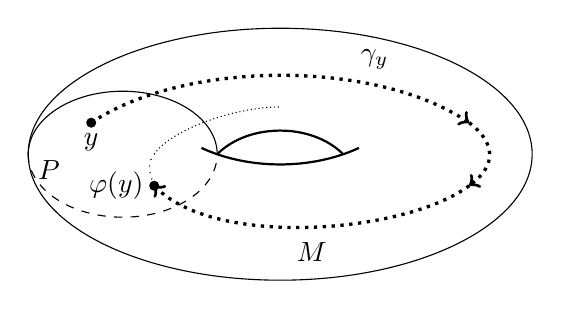
\begin{tikzpicture}[scale=.4]
    \draw (8,0) arc[start angle=0, end angle=360, x radius= 8, y radius=4];
    \draw (-2,0) arc[start angle=0, end angle=180, x radius =3, y radius=2];
    \draw[dashed] (-8,0) arc[start angle=180, end angle=360, x radius=3, y radius=2];
    \draw[thick] (-2,0) .. controls (-1,1) and (1,1) .. (2,0);
    \draw[thick] (-2.5,0.2) .. controls (-1,-0.5) and (1, -0.5)..(2.5,0.2); 
    \filldraw[black] (-6,1) circle [radius=4pt]
    (-4,-1) circle[radius=4pt];
    
    \draw[dotted, very thick,->] (-6,1) node[below]{$y$} .. controls (-3,3) and (3,3)  .. (6,1);
    
    \draw[dotted, very thick,->](6,1) ..controls (6.85555,0.3555) and (6.85555,-0.3555).. (6,-1);
    \draw[dotted, very thick,->] (6,-1)..controls (4,-2.5) and (-2,-3) ..(-4,-1) node[left]{$\varphi(y)$};
    \draw(-8,-0.5) node [right]{$P$}
    (3,3) node{$\gamma_y$};
    \draw(1,-2.5) node[below]{$M$};
    \draw[dotted] (-4,-1)..controls  (-4.2,-0.5) and (-4.2, -0.25) .. (-4,0);
    \draw[densely dotted] (-4,0) .. controls (-3.5,0.75) and (-1.5,1.5) .. (0,1.5);
\end{tikzpicture}
\caption{\footnotesize The picture illustrates how the geodesic $\gamma_y$, from $y=\gamma_y(0)\in P$, traverses along all nodal domains and turn back to $P$ the second time at $\varphi(y)=\gamma_y\left(\frac{\mathcal{N}(u)}{\sqrt{\lambda}}\right)$.}
    \label{haha}

    
    \end{figure}
    Therefore, we can conclude that $M$ is isometric to $\mathbb{R}\times_\mathbb{Z} N$ where $N$ is a compact Riemannian manifold of $\ric\geq 0$ and $\mathbb{Z}$ acts on $\mathbb{R}\times N$ by the action $k\cdot (t,x)=\left(t+k\frac{\mathcal{N}(u)\pi}{\sqrt{\lambda}},\varphi^k(x)\right)$ where $k\in \mathbb{Z},(t,x)\in \mathbb{R}\times N$ and $\varphi:N\to N$ is an isometry of $N$. 

    
\end{proof}

Turn back to our rigidity problem, we prove the Theorem \ref{main2}:


\begin{proof}[Proof of Theorem \ref{main2}]
Consider the normalized basic eigenfunction $u$ of $\lambda_1^B$ as described in Theorem \ref{main1}.

    With the assumption $\lambda_1^B=\pi^2/\d_{M/\mathcal{F}}^2$, from \ref{uu}, we get $a=0$ and hence $k=1$. Remember that in the proof of Theorem \ref{main1}, we have to let $\varepsilon\to 0$, so from \ref{uiia}, \ref{sf} and \ref{sg}, we get 
\begin{align}\label{uiiia}
    \vert\nabla\theta\vert^2=\lambda_1^B \text{ almost everywhere on }\gamma,
\end{align} where $\theta=\sin^{-1}u$. Hence, we can confirm the existence of $p\in M$ such that $\vert\nabla\sin^{-1} u(p)\vert^2=\lambda_1^B$ where $\vert u(p)\vert<1$.

Apply Theorem \ref{uoa}, we get that $M$ is isometric to a $\mathbb{R}\times_\mathbb{Z} N^{n-1}$ where $N^{n-1}$ is a compact Riemannian manifold of $\ric\geq 0$ and $\mathbb{Z}$ acts on $\mathbb{R}\times N$ by the action $k\cdot (t,x)=\left(t+k\frac{\mathcal{N}(u)\pi}{\sqrt{\lambda_1^B}},\varphi^k(x)\right)$ where $k\in \mathbb{Z},(t,x)\in \mathbb{R}\times N$ and $\varphi:N\to N$ is an isometry of $N$.  Let $\Tilde{\psi}: M\to \mathbb{R}\times_\mathbb{Z} N$ be that isometry and $\Tilde{p}:\mathbb{R}\times_\mathbb{Z}N\to \mathbb{R}/\mathbb{Z}\cong S^1\left(\frac{\mathcal{N}(u)}{2\sqrt{\lambda_1^B}}\right)$ is the induced map from the $\mathbb{Z}-$equivariant projection $p:\mathbb{R}\times N\to\mathbb{R}$ with the $\mathbb{Z}-$action on $\mathbb{R}$ is defined by the translation $k\cdot t=t+k\frac{\mathcal{N}(u)\pi}{\sqrt{\lambda_1^B}}$ where $k\in \mathbb{Z},t\in\mathbb{R}$. Also, denote $\d_1,\d_2$ as distance functions on $\mathbb{R},N$ respectively and denote $\d$ as the induced distance function on $\mathbb{R}\times_\mathbb{Z}N$. 

Consider the collection of submanifolds $\mathcal{F}'=\{\Tilde{p}^{-1}([x]): [x]\in \mathbb{R}/\mathbb{Z}\}$, where $\Tilde{p}^{-1}([x])=[(x,N)]:=\{[(x,y)]:y\in N\}$. This defines a Riemannian foliation. By identifying $\mathcal{F}$ with $\Tilde{\psi}(\mathcal{F})$, we want to show that $\mathcal{F}$ is finer than $\mathcal{F}'$. To do that, we will prove that $\Tilde{p}$ is constant on each $L\in\mathcal{F}$. Since $\vert \nabla u\vert^2=\langle \nabla u,\nabla u\rangle$ is basic (see Proposition 7 in \cite{ricardoradeschi}), $\vert \nabla u\vert^2$ is constant on any leaf $L\in \mathcal{F}$. Consider a leaf $L\in \mathcal{F}$ and $x\in L$. If $\vert\nabla u(x)\vert>0$, then $\vert \nabla u(y)\vert=\vert \nabla u(x)\vert>0$ for all $y\in L$ and the connectedness of $L$ and $M_x$ imply that $L\subset M_x$. From the construction of $M_x$ in Proposition \ref{uiiiiia}, we defined the isometry $\psi:M_x\to \left(-\frac{\pi}{2\sqrt{\lambda_1^B}},\frac{\pi}{2\sqrt{\lambda_1^B}}\right)\times N$ given by the formula $y\mapsto \left(\frac{1}{\sqrt{\lambda_1^B}}\sin^{-1}u(y),\mathcal{P}(y)\right)$. Hence, the constancy of $u$ on $L$ implies that $\psi(x)$ has the first coordinate constant on $L$ and then $\Tilde{p}$ is also constant on $L$. In the case of $\vert\nabla u(x)\vert=0$, there exists $y\in M$ such that $x\in u^{-1}(1)\cap \overline{M_y}$ or $x\in u^{-1}(-1)\cap\overline{M_y}$, and without loss of generality, assume that $x\in u^{-1}(1)\cap\overline{M_y}=V$. Then, from the proof of Theorem \ref{uoa}, we can get a local coordinate $\phi(z)=(z_1(z),z_2(z))$ on a tubular neighborhood $U=U_{r_0}(V)$ of $V$ which a chosen $r_0>0$, where 
$z_1(z)=\d(z,V)$ if $z\in M_y\cap U$ and $z_1(z)=-\d(z,V)$ if $z\in U\setminus M_y$. Notice that for every $z\in L$, $u(z)=u(x)=1$, then by the connectedness, we imply that $z\in V$ and hence $z_1(z)=\d(z,V)=0$ for every $z\in L$ and hence $\Tilde{p}$ is constant on $L$. Combine two cases, we get that $\tilde{p}$ is constant on each leaf of $\mathcal{F}$ and therefore, by identifying $\Tilde{\psi}(\mathcal{F})$ with $\mathcal{F}$, we conclude that $\mathcal{F}$ is finer than $\mathcal{F}'$.





%Here, we need to point out the detailed construction of the isometry in Proposition \ref{uiiiiia} and Theorem \ref{uoa}: the map $\psi:M_p\to\left(-\frac{\pi}{2\sqrt{\lambda_1^B}},\frac{\pi}{2\sqrt{\lambda_1^B}}\right)\times \mathcal{L}_0$ defined by $x\mapsto (\Theta(x),\mathcal{P}(x))$ has the first coordinate constant on each leaf of $\mathcal{F}$. It is because $u$ is constant on each leaf of $\mathcal{F}$ and the formula $\Theta=\frac{1}{\sqrt{\lambda_1^B}}\sin^{-1}u$ implies $\Theta$ is also constant on each leaf of $\mathcal{F}$. By the extended splitting domain process in Theorem \ref{uoa}, the constructed isometry $\Tilde{\psi}=(f,g):M\to S^1\left(\frac{\mathcal{N}(u)}{2\sqrt{\lambda_1^B}}\right)\times N$ has the property that $f$ is constant on each leaf of $\mathcal{F}$, and it means $\Tilde{\psi}(L)\subset \{\text{point}\}\times N$.
%Denote by $\mathcal{F'}$ the product singular Riemann ian foliation on $M$ with leaves of the form $\{\text{point}\}\times N$. Then the definition of $\mathcal{F'}$ tells us that each leaf of $\mathcal{F}$ is contained in some leaf of $\mathcal{F'}$ and therefore, $\mathcal{F'}$ is coarser that $\mathcal{F}$.

Let $\d_{M/\mathcal{F'}}$ be the diameter of the leaf space $M/\mathcal{F'}$. Since $M/\mathcal{F'}$ is isometric to $S^1\left(\frac{\mathcal{N}(u)}{2\sqrt{\lambda_1^B}}\right)$ and because $\mathcal{F'}$ is coarser than $\mathcal{F}$ so 
\begin{align*}
\frac{\mathcal{N}(u)}{2}\d_{M/\mathcal{F}}=\frac{\pi\mathcal{N}(u)}{2\sqrt{\lambda_1^B}}=\d_{M/\mathcal{F'}}\leq \d_{M/\mathcal{F}}.
\end{align*}and this implies $\mathcal{N}(u)\leq 2$. Therefore, $\mathcal{N}(u)=2$.
%Let $\Tilde{\psi}:M\to S^1\times N^{n-1}$ be the corresponding isometry such that for each leaf $L\in\mathcal{F}$, $\Tilde{\psi}(L)$ is contained in a leaf of $\mathcal{F'}=\{x\times N\vert x\in S^1\}$. We identify $M$ with $S^1\times N$ and $\mathcal{F}$ with $\Tilde{\psi}(\mathcal{F})=\{\Tilde{\psi}(L)\vert L\in\mathcal{F}\}$. Then we see that $\mathcal{F'}$ is coarser than $\mathcal{F}$.


Finally, we want to show that $\mathcal{F}=\mathcal{F}'$ by showing that each leaf of $\mathcal{F}'$ contains exactly one leaf of $\mathcal{F}$, which indicates the conclusion. Indeed, let $L_1$ and $L_2$ be leaves of $\mathcal{F}$ such that $L_1,L_2\subset L'_t= \Tilde{p}^{-1}([t])$. Let $s=[(t+\d_{M/\mathcal{F}},s_2)]\in \mathbb{R}\times_\mathbb{Z} N$ be a point where $s_2\in N$.

    \begin{figure}[h!]
  \centering
        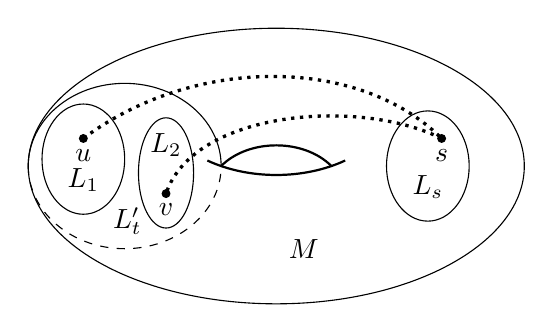
\begin{tikzpicture}[scale=.35]
    \draw (9,0) arc[start angle=0, end angle=360, x radius= 9, y radius=5];
    \draw (-2,0) arc[start angle=0, end angle=180, x radius =3.5, y radius=3];
    \draw[dashed] (-9,0) arc[start angle=180, end angle=360, x radius=3.5, y radius=3];
    \draw[thick] (-2,0) .. controls (-1,1) and (1,1) .. (2,0);
    \draw[thick] (-2.5,0.2) .. controls (-1,-0.5) and (1, -0.5)..(2.5,0.2); 
    \filldraw[black] (-7,1) circle [radius=4pt]
    (-4,-1) circle[radius=4pt];
    
    \draw[dotted, very thick] (-7,1) node[below]{$u$} .. controls (-3,4) and (3,4)  .. (6,1) node[below]{$s$};
    \draw (-5.5,0.25) arc[start angle=0, end angle=360, x radius=1.5, y radius=2];
    \draw(-7,-0.5) node{$L_1$};
    \draw (-3,-0.25) arc[start angle=0, end angle=360, x radius=1, y radius=2];
    \draw(-4,0) node[above]{$L_2$};
    \filldraw[black] (6,1) circle [radius=4pt]
    (-4,-1) node[below]{$v$};
    \draw[dotted, very thick](6,1).. controls (3,2.5) and (-3,2) .. (-4,-1);
    \draw (7,0) arc[start angle=0, end angle=360, x radius=1.5,y radius=2];
    \draw(5.5,0) node[below]{$L_s$};
    \draw (-5.4,-2) node{$L'_t$};

    
    \draw(1,-3) node{$M$};
    
  
\end{tikzpicture}
\caption{\footnotesize To show $L_1=L_2$, the idea is to prove that if $u,v$ are points that realize the distances from $s$ to each leaf $L_1,L_2$ respectively, then $u$ and $v$ must be the same point. In the picture, we see that if $L_1\neq L_2$, then $u\neq v$.}
    \label{hahaha}

    
    \end{figure}



Now, by the global equidistance, we see that  
\begin{align*}
    \d_{M/\mathcal{F}}\geq \d(L_s,L_1)=\d(s, L_1)=\d(s,u)&=\sqrt{\d_1^2(t,t+\d_{M/\mathcal{F}})+\d_2^2(s_2,u_2)}\\&=\sqrt{\d^2_{M/\mathcal{F}}+\d_2^2(s_2,u_2) },
\end{align*}where $u=[(t,u_2)]$ is some point of the leaf $L_1\subset \Tilde{p}^{-1}([t])$. This implies that $\d_2(s_2,u_2)=0$ and so $u_2=s_2$.

Similarly, there exists a point $v=[(t,v_2)]\in L_2$ such that $v_2=s_2$.

Since $u=[(t,u_2)]=[(t,s_2)]=v$ and we know the fact that $u\in L_1,v\in L_2$, so $L_1=L_2$ (See Figure \ref{hahaha}). It also means that $L'_t=\Tilde{p}^{-1}([t])$, a $\mathcal{F}$-saturated set, consists of only one leaf.

Therefore, $\mathcal{F}=\mathcal{F}'=\{\Tilde{p}^{-1}([t])\}$ and we finish the proof.



\end{proof}

%Some idea want to try
%We see that $\d_{M/\mathcal{F}}=L(\gamma)\sqrt{\lambda_1^B}=\int_\gamma\sqrt{\lambda_1^B}=\int_\gamma$ and $\vert\nabla\theta\vert^2=\lambda_1^B$ a.e.

%Especially, $\vert\nabla\theta\vert^2=\lambda_1^B$ on each $M_p=\text{component of }\{x\in M\big|\vert\nabla u(x)\vert>0\}$ containing $p$.

%We have
%\begin{align*}
 %   &\sin\left(\frac{\pi}{2}-\delta\right)=\frac{1}{1+\varepsilon}\\
  %  & A=\theta_\varepsilon^{-1}\left(\frac{\pi}{2}-\delta\right)=u^{-1}(1),B=\theta_\varepsilon^{-1}\left(-\frac{\pi}{2}+\delta\right)=u^{-1}(-1)
%\end{align*}

%Let $x\in B,y\in A$ be mentioned points in the proof of theorem 1.1 and consider $z\in A$ to be an arbitrary point. Let $\alpha$ to be the horizontal geodesic joining $L_x,L_z$. Then, we get that:
%\begin{align*}
 %   \d_{M/\mathcal{F}}\geq L(\alpha)=\d(L_x,L_z)=\d(x,L_z)\geq\d(x,A)=\d(x,L_y)=L(\gamma)=\d_{M/\mathcal{F}} 
%\end{align*}

%Hence, it implies that $\d(x,L_z)=\d(L_x,L_z)=\d_{M/\mathcal{F}}$ for every $z\in A$.

%Similarly, by working on the eigenfunction $-u$, we get $\d(L_t,L_y)=\d_{M/\mathcal{F}}$ for every $t\in B$.

%Consider a unit speed horizontal geodesic $\gamma:[0,\d_{M/\mathcal{F}}]\to M$ joining two leaves $L_x,L_y$ where $u(x)=-1$ and $u(y)=1$. Then, denote $f(t)=u(\gamma(t))$, and we see that:
%\begin{align*}
 %   \vert f'(t)\vert=\vert\langle\nabla u(\gamma(t)),\gamma'(t)\rangle\vert\leq\vert\nabla u(\gamma(t))\vert\leq\sqrt{\lambda_1^B(1-(f(t))^2)}
%\end{align*}

%Hence, for any $\varepsilon>0$, 
%\begin{align}\label{aha}
    %\pi&=\d_{M/\mathcal{F}}\sqrt{\lambda_1^B}\geq\int_{\{0\leq t\leq \d_{M/\mathcal{F}},f'(t)>0\}}\sqrt{\lambda_1^B}dt\nonumber\\
    %&\geq\int_{0}^{\d_{M/\mathcal{F}}}\frac{f'(t)}{\sqrt{1-(f(t))^2}+\varepsilon}dt\nonumber\\&=\int_{-1}^1\frac{1}{\sqrt{1-x^2}+\varepsilon}dx
%\end{align}

%Let $\varepsilon\to 0^+$, we see 
%\begin{align*}
 %   \pi\geq\int_{\{0\leq t\leq \d_{M/\mathcal{F}},f'(t)>0\}}\sqrt{\lambda_1^B}dt\geq\int_{-1}^1\frac{1}{\sqrt{1-x^2}}dx=\pi
%\end{align*}
%It follows that $f'(t)>0$ a.e $t\in (0,\d_{M/\mathcal{F}})$. Hence $f$ is strictly increasing on $[0,\d_{M/\mathcal{F}}$. From \ref{aha}, we see
%\begin{align*}
 %   \int_0^{\d_{M/\mathcal{F}}}\frac{f'(t)}{\sqrt{1-(f(t))^2}}dt=\pi
%\end{align*}
%It follows that $f'(t)=\sqrt{1-(f(t))^2}$ for $t\in (0,\d_{M/\mathcal{F}})$, and by the continuity, we have
%$$f'(t)=\sqrt{\lambda_1^B(1-(f(t))^2)}$$ for all $t\in [0,\pi]$. Hence $\lambda_1^Bf^2+(f')^2=\lambda_1^B$. With the boundary condition $f(0)=-1$ and $f(\d_{M/\mathcal{F}})=1$, we imply that
%\begin{align*}
 %   f(t)=u(\gamma(t))=-\cos\left(\frac{\pi t}{\d_{M/\mathcal{F}}}\right)=-\cos(\sqrt{\lambda_1^B}t)
%\end{align*}for $t\in [0,\d_{M/\mathcal{F}}]$.

%We prove that $\gamma$ is the integral curve of vector field $X=\nabla\theta$ pass through $p$ on $M_p$ where $p=\gamma\left(\frac{\d_{M/\mathcal{F}}}{2}\right)\in u^{-1}(0)$ and $\theta=\frac{1}{\sqrt{\lambda_1^B}}\sin^{-1} u$.

%Indeed, we know that $\vert\nabla\theta\vert=1$ so the integral curve $\alpha$ of $\nabla\theta$ is a geodesic. Hence, we need to prove that $\gamma$ and $\alpha$ at $p=\gamma\left(\frac{\d_{M/\mathcal{F}}}{2}\right)$ have the same velocity.

%We see that
%\begin{align*}
 %   \left\langle\nabla u\left(\gamma\left(\frac{\d_{M/\mathcal{F}}}{2}\right)\right),\gamma'\left(\frac{\d_{M/\mathcal{F}}}{2}\right)\right\rangle=\frac{\d}{\d t}\bigg|_{t=\frac{\d_{M/\mathcal{F}}}{2}}u(\gamma(t))=\sqrt{\lambda_1^B}
%\end{align*}

%On the other hand, we know
%\begin{align*}
 %    \left\vert\left\langle\nabla u\left(\gamma\left(\frac{\d_{M/\mathcal{F}}}{2}\right)\right),\gamma'\left(\frac{\d_{M/\mathcal{F}}}{2}\right)\right\rangle\right\vert\leq\left\vert\nabla u\left(\gamma\left(\frac{\d_{M/\mathcal{F}}}{2}\right)\right)\right\vert=\sqrt{\lambda_1^B}
%\end{align*}because $\vert\nabla u\vert^2=\lambda_1^B(1-u^2)$.

%This implies that
%\begin{align*}
 %   \gamma'\left(\frac{\d_{M/\mathcal{F}}}{2}\right)=\frac{1}{\sqrt{\lambda_1^B}}\nabla u\left(\gamma\left(\frac{\d_{M/\mathcal{F}}}{2}\right)\right)=\nabla\theta\left(\frac{\d_{M/\mathcal{F}}}{2}\right)=\alpha'\left(\frac{\d_{M/\mathcal{F}}}{2}\right)
%\end{align*}

%Another way to check that $\gamma$ is an integral curve of $X=\nabla\theta$ on $M_p$. Indeed:
%\begin{align*}
 %   \vert\nabla\theta(\gamma(t))-\gamma'(t)\vert^2&=\vert\nabla\theta(\gamma)\vert^2-2\langle\nabla\theta(\gamma(t)),\gamma'(t)\rangle+\vert\gamma'(t)\vert^2\\
  %  &=1-\frac{2\langle\nabla u(\gamma(t)),\gamma'(t)\rangle}{\sqrt{\lambda_1^B}\sqrt{1-(u(\gamma(t)))^2}}+1\\
   % &=1-\frac{2(u(\gamma(t)))'}{\sqrt{\lambda_1^B}\sqrt{1-(u(\gamma(t)))^2}}+1\\
   % &=1-\frac{2\sqrt{\lambda_1^B}\sin(\sqrt{\lambda_1^B}t)}{\sqrt{\lambda_1^B}\sqrt{1-\cos^2(\sqrt{\lambda_1^Bt})}}+1\\&=1-\frac{2\sin(\sqrt{\lambda_1^B}t)}{\sin(\sqrt{\lambda_1^B}t)}+1=0
%\end{align*}
%Hence, $\gamma'(t)=\nabla\theta(\gamma(t))=X(\gamma(t))$.



\begin{remark}
    In the case when $\mathcal{F}$ is given as the (connected) fibers of a Riemannian submersion $\pi:M\to M/\mathcal{F}$ with totally geodesic (or, more generally, minimal) fibers, if we apply Hang-Wang rigidity for the first non-zero eigenvalue of $M/\mathcal{F}$ which is also the first non-zero basic eigenvalue of $M$, then 
     we can only conclude that $M/\mathcal{F}$ is isometric to $S^1\left(\frac{1}{\sqrt{\lambda_1^B}}\right)$ without knowing the structure of $\mathcal{F}$. By proving Theorem \ref{main2}, not just $M/\mathcal{F}$, but we also understand the shape of $M$ and the structure of $\mathcal{F}$.
\end{remark}


\section{The case of Positive Ricci curvature}\label{1111}

In this section, we study a lower bound for the case of singular Riemannian foliations on a compact Riemannian manifold with the assumption of\textbf{ positive Ricci curvature. }.

We will follow the ideas that are showed in the work of Bakry-Qian (see Theorem 14, \cite{bakryqian}), and the work of Shi-Zhang \cite{shizhang} to prove Theorem \ref{main}.

\begin{lemma}[\cite{bakryqian}]\label{jjj}

For given $K>0,n>1,a,\delta<\frac{\pi}{\sqrt{K}}$, let $\lambda(K,n,\delta,a)$ be the first non-zero eigenvalue of the Neumann problem on the interval of length $\delta$, $[a,a+\delta]$, of the equation given by
\begin{align*}
   L_{K,n}v=-\lambda v\text{ on }(a,a+\delta),
\end{align*} and\begin{align*}
v'(a)=v'(a+\delta)=0,
\end{align*} where $(L_{K,n}v)(x):= v''(x)-(n-1)\sqrt{K}\tan(\sqrt{K}x)v'(x)$

Then we have two properties of $\lambda(K,n,\delta,a)$:
\begin{enumerate}[(1)]
    \item $\lambda(K,n,\delta,a)\geq \lambda(K,n,\delta,-\delta/2)$, in other words, the central interval has the lowest Neumann eigenvalue.
    \item The function $\d\mapsto \lambda(K,n,\d,-\d/2)$ is a non-increasing function.
\end{enumerate}




\end{lemma}

\begin{proof}
    To prove (1), see Theorem 13 of \cite{bakryqian}.

    For proving (2), see the discussion of eigenvalues on symmetric intervals of section 3 of \cite{bakryqian}, or the last argument in Theorem 14 of \cite{bakryqian}.
\end{proof}
%\begin{theorem}[Theorem 9 of \cite{bakryqian}]
%Assume that the operator $L$ satisfies $CD(n-1,n)$, and that $u$ is an eigenvector solution of $L(u)=-\lambda u$, with $\lambda>n$. Assume that $\min u=-1$. Consider the solution $v$ of the differential equation
%\begin{align*}
    %v''=(n-1)\tan(x) v'-\lambda v;v\left(-\frac{\pi}{2}\right)=-1,v'\left(-\frac{\pi}{2}\right)=0
%\end{align*}

%Let $b=\inf\{x>-\pi/2\vert v'(x)=0\}$ and $m=v(b)$. Then $\max u\geq m$.
%\end{theorem}

%\begin{lemma}\label{iii}
    %Given $M^n$ a compact Riemannian manifold with the Ricci curvature of $M$ is bounded below by $(n-1)K>0$.
    
   % Let $u$ be an eigenfunction of $\Delta u=-\lambda u$. Assume that $\min u=-1$. Consider the solution $v$ of the differential equation $L_{K,n}v=-\lambda v$, where $v\left(-\frac{\pi}{2\sqrt{K}}\right)=-1,v'\left(-\frac{\pi}{2\sqrt{K}}\right)=0$.

    %Let $b=\inf\left\{x>-\frac{\pi}{2\sqrt{K}}\vert v'(x)=0\right\}$ and $m=v(b)$. Then $\max u\geq m$.
%\end{lemma}

%\begin{proof}
    %See Theorem 9 of \cite{bakryqian}.
%\end{proof}

In the following lemma, we proceed exactly as in the proof of Theorem 14, \cite{bakryqian}, with the new thing is we choose a more specific geodesic to take an integral, similar to the way that is introduced in the proof of Theorem \ref{main1}.

\begin{lemma}\label{999}
    Let $M^n$ be a compact Riemannian manifold and $\mathcal{F}$ be a singular Riemannian foliation of $M$ with closed leaves and basic mean curvature. Assume the Ricci curvature of $M$ is bounded below by $(n-1)K>0$. Suppose $\lambda_1^B$ is the first basic eigenvalue of $(M/\mathcal{F})$ and $\d_{M/\mathcal{F}}$ is the diameter of the leaf space $M/\mathcal{F}$. Then $$\lambda_1^B\geq \lambda(K,n,\d_{M/\mathcal{F}},-\d_{M/\mathcal{F}}/2).$$ %where $\widehat{\lambda}(R,d,\d_{M/\mathcal{F}})$ denotes the first non zero eigenvalue of the problem
    %\begin{align*}
       % &v''-(n-1)\sqrt{K}\tan(\sqrt{K}x)=-\lambda_1^Bv\text{, on }\left(-\frac{\d_{M/\mathcal{F}}}{2},\frac{\d_{M/\mathcal{F}}}{2}\right),\\
        %&v'\left(-\frac{\d_{M/\mathcal{F}}}{2}\right)=0,v'\left(\frac{\d_{M/\mathcal{F}}}{2}\right)=0
    %\end{align*}
\end{lemma}
\begin{proof}
   Use a similar argument as in the Theorem 14 of \cite{bakryqian}: First, let $u$ be the (basic) eigenfunction with the eigenvalue $\lambda_1^B$. Similar as the argument in the introduction of the subsection \ref{888}, we can normalize $u$ and assume $u$ is the (basic) eigenfunction with the eigenvalue $\lambda_1^B$ such that $\min u=-1$ and $0<\rho=\max u\leq 1$. 

There exists an interval $[a,b]$ which has $\lambda=\lambda_1^B$ as the eigenvalue with the eigenfunction $v$ of $L_{K,n}v=-\lambda v$ with Neumann boundary conditions $v'(a)=v'(b)=0$, such that the corresponding eigenvector $v$ of the model satisfies $v(a)=-1$ and $v(b)=\rho$ (See Proposition 1, Section 3 and Theorem 9, Section 6, of \cite{bakryqian} for more detail).

  Then, apply Theorem 8 of \cite{bakryqian} for the function $g=v^{-1}\circ u$ to get that  $\vert \nabla g\vert\leq 1$. 
   
   Let $x\in M$ such that $u(x)=-1$. Choose $y$ from the level set $A=u^{-1}(\rho)$ and let $\gamma
        $ be the geodesic from $x$ to $y$ that minimizes the distance from $x$ to the $ u^{-1}(\rho)$. That gives us
        \begin{align}
            L(\gamma)=\d(x,y)=\d(x,A).
        \end{align}

        This geodesic $\gamma$ is also the shortest geodesic from $x$ to $L_y\subset A$, which means $d(x,A)=d(x,L_y)$.

        The global equidistance of $\mathcal{F}$ implies  that $\d(x,L_y)=d(L_x,L_y)$ and hence
        \begin{align}
            \d(x,y)=L(\gamma)=\d(L_x,L_y)\leq\sup_{p,q\in M}\d(L_p,L_q)=d_{M/\mathcal{F}}.
        \end{align}

        Since $\vert\nabla g\vert\leq 1$, we get that\begin{align}\label{kkk}
            \d_{M/\mathcal{F}}\geq\d(x,y)=\int_\gamma \d t\geq\left\vert\int_\gamma\nabla g\cdot \d r\right\vert=\vert g(y)-g(x)\vert=b-a.
        \end{align}

        From Lemma \ref{jjj}, we see that \begin{align*}
            \lambda_1^B=\lambda(K,n,b-a,a)\geq \lambda(K,n,b-a,-(b-a)/2).
        \end{align*}

       Because the function $\d\mapsto\lambda(K,n,\d,-\d/2)$ is non-increasing, hence, use \ref{kkk},  we get that
        \begin{align*}
            \lambda_1^B\geq\lambda(K,n,\d_{M/\mathcal{F}},-\d_{M/\mathcal{F}}/2).
        \end{align*}
\end{proof}



Finally, we are ready to prove Theorem \ref{main}
\begin{proof}[Proof of Theorem \ref{main}]
First, assume that $K>0$.

    Use Lemma \ref{999}, then we get that $\lambda_1^B\geq \lambda(K,n,\d_{M/\mathcal{F}},-\d_{M/\mathcal{F}}/2)$. Let $v$ be the corresponding eigenfunction of $\lambda(K,n,\d_{M/\mathcal{F}},-\d_{M/\mathcal{F}}/2)$ of the equation
    \begin{align*}
        L_{K,n}v=-\lambda v\text{ on }\left(-\frac{\d_{M/\mathcal{F}}}{2},\frac{\d_{M/\mathcal{F}}}{2}\right),
    \end{align*}and $v'\left(-\frac{\d_{M/\mathcal{F}}}{2}\right)=v'\left(\frac{\d_{M/\mathcal{F}}}{2}\right)=0$.

    Notice that $v$ is odd, so $v(0)=0$. Without loss of generality, we assume that $v(x)> 0$ if $x>0$.

    Recall the most important calculation from Shi-Zhang (see Lemma 2.2, \cite{shizhang})
    \begin{lemma}[Lemma 2.2 of \cite{shizhang}]\label{abcde}
        Assume $\lambda$ and $f(x),0\leq x\leq l$ satisfy that
        \begin{align*}
            f''(x)+F(x)f'(x)=-\lambda f(x),\text{ }x\in [0,l],
        \end{align*}where $F(x)$ be a differentiable function on $[0,l]$ with $F(0)=0$ and $f(x)$ satisfies the conditons $f(0)=0, f(x)>0$ when $x>0$, and $f'(l)=0$.

        Denote $F_0:=\max \{F'(x):0\leq x\leq l\}$, then we have the following estimate
        \begin{align}\label{zzz}
            \lambda\geq-s^2\left(\frac{\pi}{l}\right)^2+s\left(\left(\frac{\pi}{l}\right)^2-F_0\right).
        \end{align}for any constant $s$ such that $0<s<1$.
    \end{lemma}
    \begin{proof}[Proof of Lemma 4.4] See Lemma 2.2. \cite{shizhang}.
        
    \end{proof}
To finish the proof of Theorem \ref{main}, we consider two cases:
 
 
 \textbf{Case 1:} If $\d_{M/\mathcal{F}}=\frac{\pi}{\sqrt{K}}$, then the RHS of \ref{uuuuuu} can be written as
\begin{align*}
    4s(1-s)K+s(n-1)K=[4s(1-s)+s(n-1)]K\leq [1+(n-1)K]=nK.
\end{align*}

The inequality \ref{uuuuuu} is true, indeed, by following Lichnerowicz's estimate, we see that $\lambda_1^B\geq\lambda_1\geq nK$.

\textbf{Case 2:} If $\d_{M/\mathcal{F}}<\frac{\pi}{\sqrt{K}}$, we apply Lemma \ref{abcde} for $F(x)=-(n-1)\sqrt{K}\tan(\sqrt{K}x), f(x)=v(x),l=\d_{M/\mathcal{F}}/2,\lambda=\lambda(K,n,\d_{M/\mathcal{F}},-\d_{M/\mathcal{F}}/2)$ with an observation that
\begin{align*}
    F_0&=\max\{F'(x):0\leq x \leq\d_{M/\mathcal{F}}\}\\&=\max\{-(n-1)K\sec^2(\sqrt{K}x):0\leq x \leq\d_{M/\mathcal{F}}\}\\&=-(n-1)K,
\end{align*} and from \ref{zzz}, we have that
\begin{align*}
    \lambda_1^B&\geq\lambda(K,n,\d_{M/\mathcal{F}},-\d_{M/\mathcal{F}}/2)\\&\geq -s^2\left(\frac{2\pi}{\d_{M/\mathcal{F}}}\right)^2+s\left(\left(\frac{2\pi}{\d_{M/\mathcal{F}}}\right)^2+(n-1)K\right)\\&=4s(1-s)\frac{\pi^2}{\d_{M/\mathcal{F}}^2}+s(n-1)K.
\end{align*}





Therefore, the inequality \ref{uuuuuu} holds when $K>0$.


In the case $K=0$, notice that for every $s$ such that $0<s<1$
\begin{align*}
    4s(1-s)\frac{\pi^2}{\d_{M/\mathcal{F}}^2}+s(n-1)K=4s(1-s)\frac{\pi^2}{\d_{M/\mathcal{F}}^2}\leq\sup_{s\in (0,1)}4s(1-s)\frac{\pi^2}{\d_{M/\mathcal{F}}^2}=\frac{\pi^2}{\d_{M/\mathcal{F}}^2}.
\end{align*}

Recall Theorem \ref{main1}, then we confirm that the inequality \ref{uuuuuu} is true when $K= 0$. 
\end{proof}
\begin{remark}
    Theorem \ref{main} can be applied particularly for $s=\frac{1}{2}$ to obtain Li's type estimate:
    \begin{align}\label{litype}
        \lambda_1^B\geq\frac{\pi^2}{\d_{M/\mathcal{F}}^2}+\frac{1}{2}(n-1)K
    \end{align}

    We can actually learn more about which $s$ would give the best estimate: let $A=\frac{\pi^2}{\d_{M/\mathcal{F}}^2},B=(n-1)K$, then observe that the right hand side of the inequality \ref{uuuuuu} is a quadratic function of $s$:
    \begin{align*}
        b(s)=4s(1-s)A+sB=-4As^2+(4A+B)s
    \end{align*}.

    The only zero of $b(s)$ is $s=s_0=\frac{4A+B}{8A}$.

    Therefore, by studying the function $b(s)$ on $(0,1)$, we can see that when $n\geq 3$:
    \begin{enumerate}
        \item If $s_0<1$, which is equivalent to
        \begin{align*}
            \d_{M/\mathcal{F}}<\frac{2}{\sqrt{(n-1)}}\frac{\pi}{\sqrt{K}},
        \end{align*}then the maximum of $b(s)$ is \begin{align*}
            b(s_0)=\frac{(4A+B)^2}{16A}=A+\frac{B}{2}+\frac{B^2}{16A}=\frac{\pi^2}{\d^2_{M/\mathcal{F}}}+\frac{1}{2}(n-1)K+\frac{B^2}{16A},
        \end{align*} and it is sharper than the Li's type estimate \ref{litype}.
        \item If $s_0\geq 1$, which is equivalent to say
        \begin{align*}
            \frac{2}{\sqrt{n-1}}\frac{\pi}{\sqrt{K}}\leq\d_{M/\mathcal{F}}\leq\frac{\pi}{\sqrt{K}}
        \end{align*} (We recall the upper bound by Bonnet-Myer's Theorem), then the supremum of $b(s)$ is by letting $s\to 1^-$, and we get $\lambda_1^B\geq (n-1)K$, which is weaker than Lichnerowicz's estimate. 
    \end{enumerate}

    So, we can see that Theorem \ref{main} is a sharp estimate when considering a small diameter of the leaf space, or even better, a small diameter of $M$. In this case, the optimal one is 
    \begin{align*}
        \lambda_1^B\geq\frac{\pi^2}{\d_{M/\mathcal{F}}^2}+\frac{1}{2}(n-1)K+\frac{(n-1)^2K^2\d_{M/\mathcal{F}}^2}{16\pi^2}.
    \end{align*}
\end{remark}
\begin{remark}
When $\mathcal{F}$ is given as the (connected) fibers of a Riemannian submersion $\pi:M\to M/\mathcal{F}$ with totally geodesic (or, more generally, minimal) fibers, the basic spectrum of $M$ is turned out to be the spectrum of the base $M/\mathcal{F}$ of the submersion and $\lambda_1^B$ is the first non-zero eigenvalue $\alpha_1$ of the base $M/\mathcal{F}$. We see that if we apply directly Shi-Zhang estimate for the base $M/\mathcal{F}$ with $(n-1)K>0$ as a lower bound for the Ricci curvature, we get a weaker estimate
\begin{align*}
    \lambda_1^B=\alpha_1\geq 4s(1-s)\frac{\pi^2}{\d_{M/\mathcal{F}}^2}+s(m-1)K,
\end{align*}where $m=\dim M/\mathcal{F}$.

That is why if we want to apply Shi-Zhang estimate directly and get a better result than applying Theorem \ref{main}, we expect to have a greater lower bound $K'>K$ for the Ricci curvature of $M/\mathcal{F}$, and we want the following comparison works:
\begin{align*}
    (m-1)K'\geq (n-1)K.
\end{align*}
Unfortunately, this is not always true. We see a counterexample: Let $M=S^1\times S^2$ as a product of a unit circle and two-dimensional unit sphere and consider the projection map $\pi:S^1\times S^2\to S^2$. It is easy to see that $\ric(M)=\ric(M/\mathcal{F})=2$ and $n=3,m=2$. Hence, if we choose $K=2$ then $K'=2$ is the only choice we can get. However, in this case, the inequality $(m-1)K'\geq (n-1)K$ does not hold.

Combine with the original version of Shi-Zhang estimate in the case of a foliation given by points, we can say that Theorem \ref{main} is indeed optimal.


\end{remark}

%\section{An estimate for gradients of eigenfunctions}

%Let us recall the nice results in \cite{bakryqian} for the special case of the Laplace-Beltrami operator $L=\Delta$ that we will use for our main theorem later:

%Let $M$ be a connected $n$-dimensional Riemannian  manifold and assume that $\ric\geq R=(n-1)K$.

%Let $u$ be a real eigenfunction of $\Delta$ with respect to the eigenvalue $\lambda$, i.e.
%$$\Delta u=-\lambda u$$

%Consider a solution $v$ of the equation 
%\begin{align}\label{v}
  %v''(x)-\sqrt{K}\tan(\sqrt{K}x)v'(x)=-\lambda v  
%\end{align}on some interval $(a,b)$ with $v'(a)=v'(b)=0,v'>0$ on $(a,b)$.



%In the  we have that
%\begin{theorem}
 %   If $v$ is a solution of the equation \ref{v} with the same eigenvalue $\lambda$ of $u$ that satisfies
  %  $$[\min u,\max u]\subset [\min v,\max v]$$
   % Then, we get that
    %\begin{align*}
     %   \vert \nabla u\vert^2\leq(v'\circ v^{-1})^2(u)
    %\end{align*}
    %By using the change of variable formula, we can rewrite the estimate above as
    %\begin{align*}
     %   \vert \nabla (v^{-1}\circ u)\vert^2\leq 1
    %\end{align*}
    
%\end{theorem}
%\begin{proof}
 %   See the \textbf{Theorem 8} of Bakry-Qian \cite{bakryqian} (pages 130 - 134).
%\end{proof}

%Now we are good to prove the main theorem in the next section.

%    \section{a lower bound for the First Basic Eigenvalue}

%In this section, we will prove the main theorem \ref{main}.
%\begin{proof}
%Let $u\in C^\infty_B(M)$ be a basic eigenfunction with $\Delta u=-\lambda_1^B u$. Since $\lambda_1^B\geq \lambda_1>0$, so by the Green's theorem, we will get that $\int_M{u \dvol}=0$. Because $u$ is nonzero, so we can  imply that $\max u>0>\min u$.

 %   If $\max u\geq -\min u$, then we can consider new function $v=-u/\max u$ such that $\Delta v=-\lambda_1^Bv$ and $\min v=-1,0<\max v\leq 1$. Otherwise, we consider the new function $v=-u/\min u$, and then $\Delta v=-\lambda^B_1 v$ and $\min v=1,-1\leq \max v<0$. Therefore, by rescaling (we still get the ``basic" property after rescaling), without loss of generality, we can assume that $u$ is the basic eigenfunction   with respect to $\lambda_1^B$ such that
  %  $$-1=\min u<0<\max u=k,0<k\leq 1$$

   % Then, we may use the results (9), (11), and (10): There exists an interval $[a,b]$ which has $\lambda=\lambda_1^B$ as an eigenvalue for the left hand side operator of \ref{v} with the corresponding eigenfunction $v$ of the model satisfies that $v(a)=-1,v(b)=k$.

    %Now, apply the main comparison result (8) of Section 6: the function $g=v^{-1}\circ u$ is such that $\vert\nabla g\vert\leq 1$. Consider $x\in M$ such that $u(x)=-1$ and let $\gamma:[0,1]\to M$ be the shortest geodesic joining $x$ and some point $y\in L_y$ such that $u(y)=k$ and the length of $\gamma$ is equal to $\d(x,y)=\d(x,L_y)$ because of the compactness of $L_y$. Since we are working on a singular Riemannian foliation with closed leaves, then by the global equidistant of leaves, we have that
    %$$\d(x,y)=\d(x,L_y)=\d(L_x,L_y)\leq\sup_{p,q\in M}\d(L_p,L_q)=d_{M/\mathcal{F}}$$

    %Hence, we get that
    %\begin{align}
     %   d_{M/\mathcal{F}}\geq d(x,y)\geq g(x)-g(y)=b-a
    %\end{align}

    %Use the Theorem 13 of Section 7 to obtain
    %\begin{align}
     %   \lambda_1^B=\lambda
    %\end{align}

%\end{proof}


\printbibliography

\end{document}
